\section{Pojam funkcije. Crtanje grafa funkcije}

\begin{definition}
Neka su $S$ i $S'$ dva neprazna skupa. Ako je svakom elementu $x\in S$ pridružen jedinstven element $f(x)\in S'$, onda kažemo da je zadana \textbf{funkcija} $f$ sa skupa $S$ u skup $S'$, ili kraće $f : S\to S'$. Skup $\mathcal{R}(f)=\left\{ f(x) : x\in S\right\}$ zove se \textbf{slika} od $f$. Skup $S$ zove se \textbf{domena} od $f$.
\end{definition}

Kao i prije, ove definicije nisu stroge, ali su za naše svrhe u redu.

\begin{definition}
Neka su $A, A_0$ i $B$ neprazni skupovi i neka su zadane $f : A\to B$ i $f_0 : A_0\to B$. Kažemo da je $f_0$ \textbf{restrikcija} funkcije $f$ na skup $A_0$ ako je $f_0(x)=f(x)$ za svaki $x\in A_0$, te pišemo $f_0=f|_{A_0}$. Kažemo i da je $f$ \textbf{proširenje} funkcije $f_0$ na skup $A$ ako je $f_0$ restrikcija funkcije $f$ na skup $A_0$. 
\end{definition}

\begin{remark}
Na nekim mjestima ćemo funkciju $f : S\to \mathbb{R}$, gdje je $\emptyset\neq S\subseteq \mathbb{R}$ samo navesti u kraćem obliku $x\mapsto f(x)$, u nadi da su domena i kodomena jasne iz konteksta (ili ako je kodomena nebitna). U tom slučaju govorimo o \textit{funkcijama zadanima formulom}. Tako npr. $x\mapsto 2x+1$ predstavlja funkciju $f : \mathbb{R}\to \mathbb{R}$, $f(x)=2x+1$. (Uočite da je ovdje jedina kodomena koja ima smisla upravo $\mathbb{R}$, jer je $\mathcal{R}(f)=\mathbb{R}$ i $\mathcal{R}(f)$ je podskup kodomene).
\end{remark}

\begin{definition}[Operacije s funkcijama]
Neka je $S$ neprazan skup i neka su zadane $f, g : S\to \mathbb{R}$. Tada definiramo $f+g, fg, \alpha f : S\to \mathbb{R}$ formulama
\begin{gather*}
(f+g)(x):=f(x)+g(x),\;\;(fg)(x)=f(x)g(x),\;\forall x\in S\\
(\alpha f)(x)=\alpha f(x).\;\forall x\in S.
\end{gather*}
Ako je i $g(x)\neq 0$ za sve $x\in S$, onda definiramo i $\dfrac{f}{g}$ formulom $$\left(\dfrac{f}{g}\right)(x)=\dfrac{f(x)}{g(x)},\;\;\forall x\in S.$$
\end{definition}

Nadamo se da ste se u srednjoj školi susreli s crtanjem grafova raznih funkcija. U ovoj točki pokazujemo "trikove" koje možemo upotrijebiti da bismo brže nacrtali graf neke funkcije. Ovo će biti osobito korisno u narednim točkama, gdje će crtanje grafa biti korisno u rješavanju zadataka. U skladu s time, promotrimo sljedeću napomenu.
\begin{remark}
\label{graphrem}
Neka je zadana $f : S\to \mathbb{R}$, gdje je $S\subseteq \mathbb{R}$ i neka je $c\in \mathbb{R}$.
\begin{itemize}
\item Graf funkcije $x\mapsto f(x)+c$ za $x\in S$ je graf funkcije $f$ pomaknut vertikalno za $|c|$. Ako je $c>0$, pomaknut je prema gore, a ako je $c<0$, pomaknut je prema dolje.
\item Ako je $c>0$, onda graf funkcije $x\mapsto cf(x)$ za $x\in S$ se dobiva dilatacijom grafa funkcije $f$ u smjeru prema osi $y$. Ako je $c>1$, graf će biti rastegnut, a ako je $c<1$, on će biti stisnut.
\item Graf funkcije $x\mapsto -f(x)$ za $x\in S$ je graf funkcije $f$ dobiven zrcaljenjem u odnosu na os $x$.
\item Graf funkcije $x\mapsto f(x+c)$ za $x\in S$ je graf funkcije $f$ dobiven horizontalnom translacijom za $|c|$ jediničnih dužina. Ako je $c>0$, translatiramo ga ulijevo, a ako je $c<0$, translatiramo ga udesno.
\item Ako je $c>0$, onda je graf funkcije $x\mapsto f(cx)$ za $x\in S$ graf funkcije $f$ dilatiran u smjeru $x$ osi. Ako je $c<1$, graf će biti rastegnut, a ako je $c>1$, on će biti stisnut.
\item Graf funkcije $x\mapsto f(-x)$ za $x\in S$ je graf funkcije $f$ dobiven zrcaljenjem s obzirom na os $y$.
\item Graf funkcije $x\mapsto |f(x)|$ za $x\in S$ je graf funkcije $f$ dobiven tako da sve njegove dijelove koji su ispod osi $x$ zrcalimo u odnosu na os $x$, a ostale dijelove ostavimo nepromijenjene.
\item Neka je zadana $g : S\to \mathbb{R}$. Tada su grafovi funkcija $f+g$, $fg$ dobiveni tako da za svaki $x\in S$ gledamo vrijednost funkcija $f(x)$ i $g(x)$ i ta dva broja zbrojimo, odnosno pomnožimo. Ovo je direktna posljedica definicija operacija s funkcijama.
\item Ako za funkciju $g : S\to \mathbb{R}$ vrijedi $g(x)\neq 0$ za sve $x\in S$, onda funkciju $\dfrac{f}{g}$ dobivamo tako da $f$ i $g$ podijelimo "po točkama", analogno kao u prethodnoj natuknici.
\end{itemize}
\end{remark}

\begin{exercise}
\label{exgraph1}
Nacrtajte graf funkcije $f: \mathbb{R}\to \mathbb{R}$, gdje je
\begin{itemize}
\item[a)] $f(x)=3x^2+4x+1$, 
\item[b)] $f(x)=\abs{|x|-4}$.
\end{itemize}
\end{exercise}
\begin{proof}[Rješenje] a) Nadamo se da je crtanje grafa kvadratne funkcije poznato otprije, ali za svaki slučaj ćemo to ovdje pokazati. Pri crtanju kvadratne funkcije korisno nam je znati njezino tjeme, nultočke, te eventualno još neke njezine točke. Možemo se koristiti činjenicom i da je ona simetrična s obzirom na njezinu os simetrije.\footnote{Os simetrije parabole definira se kao pravac koji prolazi kroz fokus parabole, a okomit je na njezinu direktrisu.} 

Već smo pokazali (v. zadatak \ref{tjeme}) da je tjeme kvadratne funkcije $x\mapsto ax^2+bx+c$ (gdje je $a\neq 0$) točka
$$T(x_0, y_0)=\left(-\dfrac{b}{2a}, \dfrac{4ac-b^2}{4a}\right),$$
i to minimum ako je $a>0$, a maksimum ako je $a<0$. Dakle, uvrštavanjem ovih podataka dobivamo da je tjeme parabole u točki $\left(-\dfrac{2}{3}, -\dfrac{1}{3}\right)$, gdje je $-\dfrac{1}{3}$ najmanja vrijednost koju funkcija postiže.

Nadalje, njezine nultočke su rješenja jednadžbe $3x^2+4x+1=0$, dakle $x=-1$ i $x=-\dfrac{1}{3}$. Pored toga, vrijedi $f(0)=1$, $f\left(\dfrac{1}{2}\right)=\dfrac{7}{4}$. Sad uz ove podatke nije teško nacrtati graf funkcije.

b) Primijenit ćemo napomenu \ref{graphrem}.
\begin{itemize}
\item Promotrimo graf funkcije $x\mapsto x$, čiji graf je prikazan točkasto-iscrtkanom linijom.
\item Tada je graf funkcije $x\mapsto |x|$ dobiven zrcaljenjem cijelog dijela grafa funkcije $x\mapsto x$ ispod osi $x$ u odnosu na os $x$, a ostali dijelovi su nepromijenjeni. Njezin graf je na slici \ref{gr1} prikazan točkastom linijom.
\item Graf funkcije $x\mapsto |x|-4$ je dobiven translacijom grafa funkcije $x\mapsto |x|$ četiri jedinične dužine prema dolje. Njezin graf je na slici $\ref{gr1}$ prikazan iscrtkanom linijom.
\item Graf funkcije $x\mapsto \abs{|x|-4}$ je dobiven zrcaljenjem cijelog dijela grafa funkcije $x\mapsto |x|-4$ ispod osi $x$ u odnosu na os $x$, a ostali dijelovi su nepromijenjeni. Njezin graf je na slici \ref{gr1} prikazan punom linijom.
\end{itemize}
\end{proof}
\newpage
\begin{figure}[ht]
\begin{subfigure}[t]{.5\textwidth}
\centering
\begin{tikzpicture}
\begin{axis}[axis lines=middle,xlabel=$x$,ylabel=$y$,xmin=-4,xmax=4,ymin=-1,ymax=7.5, smooth, samples=200]

\addplot[thick,color=black,domain=-3:4] {3*x^2+4*x+1};
\node[circle,fill,inner sep=2pt] at (axis cs:-2/3,-1/3) {};
\node[circle,fill,inner sep=2pt] at (axis cs:-1,0) {};
\node[circle,fill,inner sep=2pt] at (axis cs:-1/3,0) {};
\node[circle,fill,inner sep=2pt] at (axis cs:0,1) {};
\node[circle,fill,inner sep=2pt] at (axis cs:1/2,3.75) {};
\end{axis}
\end{tikzpicture}
\caption*{Graf funkcije $x\mapsto 3x^2+4x+1$}
\end{subfigure}%
\begin{subfigure}[t]{.5\textwidth}
\centering
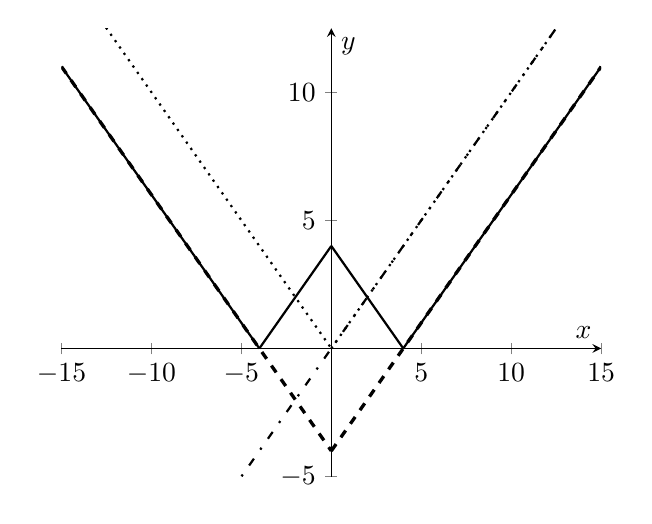
\begin{tikzpicture}
\begin{axis}[axis lines=middle,xlabel=$x$,ylabel=$y$,xmin=-15,xmax=15,ymin=-5,ymax=12.5]

\addplot[thick,color=black,domain=4:15] {x-4};
\addplot[thick,color=black,domain=0:4] {4-x};
\addplot[thick,color=black,domain=-15:-4] {-x-4};
\addplot[thick,color=black,domain=-4:0] {4+x};
\addplot[thick,loosely dashdotted,color=black,domain=-15:15] {x};

\addplot[thick,color=black, dotted,domain=0:15] {x};
\addplot[thick,color=black, dotted,domain=-15:0] {-x};
\addplot[very thick,color=black, dashed,domain=0:15] {x-4};
\addplot[very thick,color=black, dashed,domain=-15:0] {-x-4};
\end{axis}
\end{tikzpicture}
\caption*{Graf funkcije $x\mapsto \abs{|x|-4}$}
\end{subfigure}
\caption{\label{gr1} Grafovi funkcija iz zadatka \ref{exgraph1}} 
\end{figure}
\begin{exercise}
\label{exgraph2}
Nacrtajte graf funkcije $x\mapsto f(x)$, gdje je
\begin{itemize}
\item[a)] $f(x)=\dfrac{x-5}{x+5}$,
\item[b)] $f(x)=e^{|x|}$.
\item[c)] $f(x)=x-\lfloor x\rfloor$.
\end{itemize}
\end{exercise}
\begin{proof}[Rješenje] a) Uočimo da je
$$\dfrac{x-5}{x+5}=\dfrac{x+5-10}{x+5}=1-\dfrac{10}{x+5}.$$
\begin{itemize}
\item Promotrimo graf funkcije $x\mapsto -\dfrac{10}{x}$ (Prikazan točkastom linijom).
\item Tada je graf funkcije $x\mapsto -\dfrac{10}{x-5}$ dobiven translacijom grafa funkcije $x\mapsto \dfrac{10}{x}$ pet jediničnih dužina udesno (Prikazan iscrtkanom linijom).
\item Konačno, graf funkcije $x\mapsto \dfrac{x-5}{x+5}=1-\dfrac{10}{x+5}$ je dobiven translacijom grafa funkcije $x\mapsto -\dfrac{10}{x-5}$ jednu jediničnu dužinu prema gore.
\end{itemize}

b) Uočimo da je
$$e^{|x|}=\begin{cases}
e^x, & x\geq 0, \\
e^{-x}, & x<0.
   \end{cases}$$
Uz ovaj podatak nije teško nacrtati graf ove funkcije. Naime, desno od osi $y$ on će biti identičan grafu funkcije $x\mapsto e^x$, a lijevo od osi $y$ bit će identičan grafu funkcije $x\mapsto e^{-x}$, koji nastaje zrcaljenjem grafa funkcije $x\mapsto e^x$ u odnosu na os $y$. Na slici \ref{gr2} graf funkcije $x\mapsto e^{|x|}$ prikazan je punom linijom. Graf funkcije $x\mapsto e^x$ (odnosno $x\mapsto e^{-x}$), na mjestima gdje se on ne podudara s grafom funkcije $x\mapsto e^{|x|}$, prikazan je točkastom (odnosno iscrtkanom) linijom.
\begin{figure}[ht]
\begin{subfigure}{.5\textwidth}
\centering
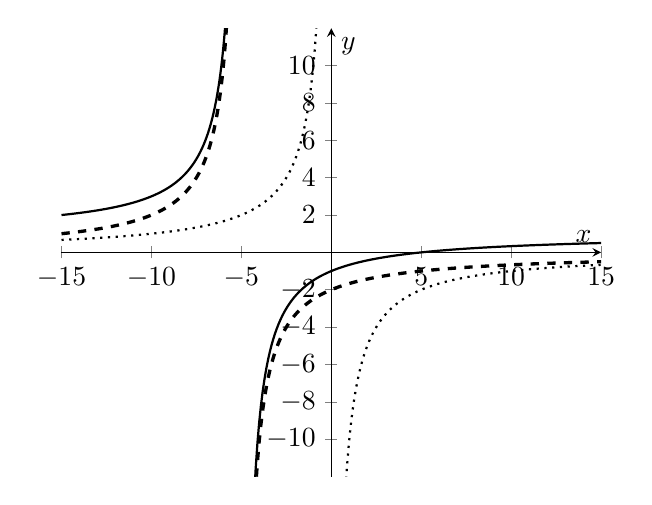
\begin{tikzpicture}
\begin{axis}[axis lines=middle,xlabel=$x$, ytick={-10,-8,-6,-4,-2, 2, 4, 6, 8, 10},ylabel=$y$,xmin=-15,xmax=15,ymin=-12,ymax=12, samples=200]

\addplot[thick,dotted,color=black,domain=-15:-0.5] {-10/x};
\addplot[thick,dotted,color=black,domain=0.5:15] {-10/x};

\addplot[very thick,dashed,color=black,domain=-15:-5.5] {-10/(x+5)};
\addplot[very thick,dashed,color=black,domain=-4.5:15] {-10/(x+5)};

\addplot[thick,color=black,domain=-15:-5.5] {(x-5)/(x+5)};
\addplot[thick,color=black,domain=-4.5:15] {(x-5)/(x+5)};
\end{axis}
\end{tikzpicture}
\caption*{Graf funkcije $x\mapsto \dfrac{x-5}{x+5}$}
\end{subfigure}%
\begin{subfigure}{.5\textwidth}
\centering
\begin{tikzpicture}
\begin{axis}[axis lines=middle,xlabel=$x$,ylabel=$y$,xmin=-4,xmax=4,ymin=-1,ymax=7.5, smooth, samples=200]

\addplot[thick,dotted,color=black,domain=-4:0] {e^x};
\addplot[very thick,dashed,color=black,domain=0:4] {e^(-x)};
\addplot[thick,color=black,domain=0:4] {e^x};
\addplot[thick,color=black,domain=-4:0] {e^(-x)};
\end{axis}
\end{tikzpicture}
\caption*{Graf funkcije $x\mapsto e^{|x|}$ \phantom{$\dfrac{2}{3}$}}
\end{subfigure}
\caption{\label{gr2} Grafovi funkcija iz zadatka \ref{exgraph2} a) i b)}
\end{figure}

c) Na slici \ref{gr3} prikazan je točkastom linijom graf funkcije $x\mapsto x$ i iscrtkanom linijom graf funkcije $x\mapsto -\lfloor x\rfloor$. Prema napomeni \ref{graphrem}, graf funkcije $x\mapsto x-\lfloor x \rfloor$ (prikazan punom linijom) bit će dobiven tako da za proizvoljnu točku $x\in \mathbb{R}$ zbrojimo vrijednosti te dvije funkcije u točki $x$.
\begin{figure}[ht]
\begin{center}
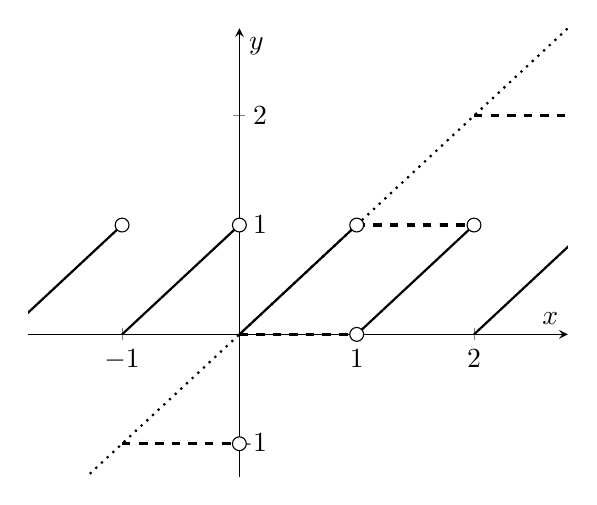
\begin{tikzpicture}
\begin{axis}[axis lines=middle,
    yticklabel style = {xshift=0.55cm},
    xlabel=$x$,ylabel=$y$,xmin=-1.8,xmax=2.8,ymin=-1.3,ymax=2.8]

\addplot[very thick,dashed,color=black,domain=0:1] {0};
\addplot[very thick,dashed,color=black,domain=1:2] {1};
\addplot[very thick,dashed,color=black,domain=2:3] {2};
\addplot[very thick,dashed,color=black,domain=-1:0] {-1};

\addplot[thick,color=black,domain=0:1] {x};
\addplot[thick,color=black,domain=1:2] {x-1};
\addplot[thick,color=black,domain=2:3] {x-2};
\addplot[thick,color=black,domain=-1:0] {x+1};
\addplot[thick,color=black,domain=-2:-1] {x+2};
\addplot[thick,dotted,color=black,domain=-2:3] {x};

\node[circle,draw=black, fill=white, inner sep=0pt,minimum size=5pt] at (1, 1) {};
\node[circle,draw=black, fill=white, inner sep=0pt,minimum size=5pt] at (2, 1) {};
\node[circle,draw=black, fill=white, inner sep=0pt,minimum size=5pt] at (3, 1) {};
\node[circle,draw=black, fill=white, inner sep=0pt,minimum size=5pt] at (0, 1) {};
\node[circle,draw=black, fill=white, inner sep=0pt,minimum size=5pt] at (-1, 1) {};
\node[circle,draw=black, fill=white, inner sep=0pt,minimum size=5pt] at (1, 0) {};
\node[circle,draw=black, fill=white, inner sep=0pt,minimum size=5pt] at (0, -1) {};

\end{axis}
\end{tikzpicture}
\end{center}
\caption{\label{gr3} Graf funkcije iz zadatka \ref{exgraph2} c)}
\end{figure}
\end{proof}
\begin{exercise} Neka je $f : \mathbb{R}\to \mathbb{R}$, $f(x)=\sin{x}$. Graf funkcije $f$ je zrcaljen po osi $y$, zatim je pomaknut za dvije jedinične dužine udesno, a potom je skaliran u odnosu na ishodište, te je koeficijent tog skaliranja (homotetije) $\dfrac{1}{2}$. Graf koje funkcije je novodobiveni skup?
\end{exercise}
\begin{proof}[Rješenje]
Zrcaljenjem dobivamo $x\mapsto -\sin{x}$, pomakom za dvije jedinične dužine udesno dobivamo $x\mapsto -\sin(x-2)$, dilatacijom po $x$ dobivamo $x\mapsto -\sin\left(2x-2\right)$, a dilatacijom po $y$ imamo $x\mapsto \dfrac{1}{2}\sin(2x-2)$. Prema tome novodobiveni skup je graf funkcije $x\mapsto \dfrac{1}{2}\sin(2x-2)$.
\end{proof}

\section{Injekcija, surjekcija i bijekcija. Slika i praslika skupa}

\begin{definition}
Neka su $S$ i $S'$ neprazni skupovi. Funkcija $f : S\to S'$ je
\begin{itemize}
\item \textbf{injekcija} ako za sve $x$, $y\in S$ vrijedi $$f(x)=f(y)\Rightarrow x=y.$$
\item \textbf{surjekcija} ako za sve $y\in S'$ postoji bar jedan $x\in S$ takav da je $f(x)=y$ (tj. vrijedi $S'=\mathcal{R}(f)$).
\item \textbf{bijekcija} ako je injekcija i surjekcija.
\end{itemize}
\end{definition}

\begin{exercise}
Neka je $f : \mathbb{R}^+\to \langle 1, \infty\rangle $ zadana formulom $f(x)=1+\dfrac{1}{x}$. Dokažite da je $f$ bijekcija.
\end{exercise}
\begin{proof}[Rješenje]
Dokažimo da je $f$ injekcija. Neka su $x, y\in \langle 1, \infty\rangle$ takvi da vrijedi $$1+\dfrac{1}{x}=1+\dfrac{1}{y}.$$ Zbog $x$, $y\neq 0$ pojednostavljivanjem i množenjem dobivamo $x=y$. 

Dokažimo da je $f$ surjekcija. Neka je $y\in \langle 1, \infty\rangle$ proizvoljan. Treba dokazati da tada postoji bar jedan $x$ takav da je $$y=1+\dfrac{1}{x}.$$ No ovo je zbog $x\neq 0$ i $y-1\neq 0$ ekvivalentno s $$x=\dfrac{1}{y-1}.$$ Zaista, $\dfrac{1}{y-1}$ je upravo jedan (i jedini) takav $x$.
\end{proof}
\begin{remark}
Lako se vidi sljedeća formulacija definicije bijekcije: $f : S\to S'$ je bijekcija ako i samo ako za svaki $y\in S'$ postoji i jedinstven je $x\in S$ takav da je $y=f(x)$. Prema tome, u prethodnom zadatku prvi dio rješenja je zapravo suvišan.
\end{remark}

\begin{exercise}
Dokažite da je $f : \mathbb{R}\to \langle 0, 1]$ zadana formulom $f(x)=\dfrac{1}{x^2+1}$ surjekcija. Je li i injekcija?
\end{exercise}
\begin{proof}[Rješenje]
Neka je $y\in \langle 0, 1]$. Treba dokazati da postoji bar jedan $x\in \mathbb{R}$ takav da je $$y=\dfrac{1}{1+x^2}.$$ No to je ekvivalentno s $$x^2=\dfrac{1}{y}-1.$$ 
Očito je $x=\sqrt{\dfrac{1}{y}-1}$ jedan $x$ koji zadovoljava tvrdnju. Nadalje, $f$ nije injekcija, jer je $-1\neq 1$ i $f(1)=f(-1)$.
\end{proof}
\begin{exercise} \textbf{}
\label{bijexmp}
\begin{itemize}
\item[a)] Odredite neku bijekciju (ako postoji) s $\mathbb{N}$ u $\mathbb{N}\setminus\{1, 2\}$.
\item[b)] Odredite neku bijekciju (ako postoji) s $\mathbb{N}$ s $[0, 1]$ u $[1, 3]$.
\item[c)] Odredite neku bijekciju (ako postoji) s $\mathbb{N}$ s $[0, 1]$ u $[0, 1\rangle$.
\item[d)] Odredite neku bijekciju (ako postoji) s $\mathbb{R}$ u skup svih funkcija s $\mathbb{R}$ u $\mathbb{R}$ (Taj skup nazivamo $\mathbb{R}^\mathbb{R}$).
\end{itemize}
\end{exercise}
\begin{proof}[Rješenje]
a) Neka je zadana $f : \mathbb{N}\to \mathbb{N}\setminus \{1, 2\}$, $f(n)=n+2$ (Ideja je "pomaknuti" svaki broj za $2$ udesno). Uvjerite se da je ova funkcija zaista bijekcija.

b) Ideja će biti uzeti linearnu funkciju čiji graf prolazi kroz točke $(0, 1)$ i $(1, 3)$ i promotriti njezinu restrikciju na segment $[0, 1]$. Uzmimo $f :[0, 1]\to [1, 3]$, $f(x)=2x+1$. Nije teško pokazati da je ova funkcija zaista bijekcija.

c) Promotrimo funkciju $f : [0, 1]\to [0, 1]$, $f(x)=x$. Ona je očito bijekcija s $[0, 1]$ na $[0, 1]$. Ideja će sada biti nju izmijeniti tako da $f(1)$ bude neki broj iz skupa $[0, 1\rangle$. Doduše, ako to napravimo, funkcija više neće biti injekcija. Zaista, znamo da je $f(f(1))=f(1)$, pa kad bi ona bila injekcija bilo bi $f(1)=1$, što nije točno. Dakle, da bi izbjegli situaciju gdje funkcija poprima dvije jednake vrijednosti, moramo je izmijeniti i za $x=f(1)$. Injektivnost će se opet "pokvariti", ali ćemo tada funkciju moći opet izmijeniti u točki koja "kvari" injektivnost. Ovaj postupak ponavljamo u beskonačnost. Zato ima smisla promotriti npr. funkciju $g : [0, 1]\to [0, 1\rangle$,

$$g(x)=\begin{cases}
x, &\;x\notin S,\\[2pt]
\dfrac{x}{2}, &\; x\in S,
\end{cases}$$
gdje je $S=\left\{\dfrac{1}{2^n} : n\in \mathbb{N}_0\right\}$.

Tvrdimo da je $g$ injekcija. Zaista, neka su $x, y\in [0, 1\rangle$ takvi da je $f(x)=f(y)$. Uočimo da ako je $x\in S$ ako i samo ako je $f(x)\in S$, pa ako je $f(x)=f(y)$, onda su ili $x, y$ oboje u $S$, ili oboje nisu u $S$. U oba slučaja je očigledno $x=y$.

Tvrdimo da je $g$ i surjekcija. Zaista, neka je $y\in [0, 1\rangle$ proizvoljan. Ako je $y\notin S$, onda je $f(y)=y$, ako je $y\in S$, onda postoji $p\in \mathbb{N}$ takav da je $y=\dfrac{1}{2^p}$. No tada je $$g\left(\dfrac{1}{2^{p-1}}\right)=\dfrac{1}{2^p},$$
gdje je $\dfrac{1}{2^{p-1}}\in S$, budući da je $y\neq 1$.

\begin{figure}[ht]
\begin{center}
\begin{tikzpicture}
\begin{axis}[axis lines=middle,   xlabel=$x$,ylabel=$y$,xmin=-0.2,xmax=1.2,ymin=-0.2,ymax=1.2]

\addplot[thick,color=black,domain=0:1] {x};

\node[circle,draw=black, fill=white, inner sep=0pt,minimum size=5pt] at (1, 1) {};
\node[circle,draw=black, fill=white, inner sep=0pt,minimum size=5pt] at (0.5, 0.5) {};
\node[circle,draw=black, fill=white, inner sep=0pt,minimum size=5pt] at (0.25, 0.25) {};
\node[circle,draw=black, fill=white, inner sep=0pt,minimum size=5pt] at (1/8, 1/8) {};
\node[circle,draw=black, fill=white, inner sep=0pt,minimum size=5pt] at (1/16, 1/16) {};
\node[circle,draw=black, fill=white, inner sep=0pt,minimum size=5pt] at (1/32, 1/32) {};
\node[circle,draw=black, fill=white, inner sep=0pt,minimum size=5pt] at (1/64, 1/64) {};

\node[circle,fill,inner sep=2pt] at (axis cs:1, 0.5) {};
\node[circle,fill,inner sep=2pt] at (axis cs:0.5, 0.25) {};
\node[circle,fill,inner sep=2pt] at (axis cs:0.25, 1/8) {};
\node[circle,fill,inner sep=2pt] at (axis cs:1/8, 1/16) {};
\node[circle,fill,inner sep=2pt] at (axis cs:1/16, 1/32) {};
\node[circle,fill,inner sep=2pt] at (axis cs:1/32, 1/64) {};
\node[circle,fill,inner sep=2pt] at (axis cs:1/64, 1/128) {};
\end{axis}
\end{tikzpicture}
\end{center}
\caption{\label{exbij} Graf funkcije iz zadatka \ref{bijexmp} c)}
\end{figure}

d) Tvrdimo da takva bijekcija ne postoji. Zaista, pretpostavimo da postoji bijekcija $f : \mathbb{R}\to \mathbb{R}^{\mathbb{R}}$. Tada je ona surjekcija, što znači da za svaki $y\in \mathbb{R}^{\mathbb{R}}$ postoji $x_0\in \mathbb{R}$ takav da je $f(x_0)=y$, što povlači da je $f(x_0)(x_0)=y(x_0)$. No to očito ne vrijedi ako promotrimo funkciju $y : \mathbb{R}\to \mathbb{R}$ definiranu formulom $y(x)=f(x)(x)+1$, za svaki $x\in \mathbb{R}$.
\end{proof}
\begin{definition}
\label{monotonic}
Neka je $S\subseteq \mathbb{R}$ neprazan, te $x, y\in S$. Kažemo da je funkcija $f : S\to \mathbb{R}$ \textbf{monotono rastuća} (kraće: rastuća) ako vrijedi $x<y\Rightarrow f(x)\leq f(y)$, \textbf{strogo rastuća} ako vrijedi $x<y\Rightarrow f(x)<f(y)$, \textbf{monotono padajuća} (kraće: padajuća) ako vrijedi $x<y\Rightarrow f(x)\geq f(y)$, \textbf{strogo padajuća} ako vrijedi $x<y\Rightarrow f(x)>f(y)$.
\end{definition}
\begin{remark}
Neka su $S, S'\subseteq \mathbb{R}$ neprazni i neka je zadana $f : S\to S'$. Ako je $f$ strogo monotona (tj. strogo rastuća ili strogo padajuća), ona je injekcija.
\end{remark}
\begin{exercise}
Zadana je $f : \mathbb{R}\to \mathbb{R}$, $f(x)=e^{-2x}$. Dokažite da je $f$ injekcija koristeći se činjenicom da je strogo monotona.
\end{exercise}
\begin{proof}[Rješenje]
Iz grafa se vidi da je $f$ strogo padajuća. 
\begin{figure}[ht]
\begin{center}
\begin{tikzpicture}
\begin{axis}[axis lines=middle, xlabel=$x$,ylabel=$y$,xmin=-1.8,xmax=3.2,ymin=-0.5,ymax=3.8, samples=150]


\addplot[thick,color=black,domain=-1:3.3] {e^(-2*x)};

\end{axis}
\end{tikzpicture}
\end{center}
\caption{\label{grexp} Graf funkcije $x\mapsto e^{-2x}$}
\end{figure}

Zaista, treba pokazati da za sve $x, y\in \mathbb{R}$ vrijedi
\begin{gather}
\label{ineq1}
x<y\Rightarrow e^{-2y}<e^{-2x}.
\end{gather}
Uočimo da, kako je $e^x\geq 0$ za sve $x\in \mathbb{R}$ i $x\mapsto x^2$ i $x\mapsto \sqrt{x}$ strogo rastuće funkcije, vrijedi
$$e^{-2y}<e^{-2x}\Leftrightarrow \dfrac{1}{\left(e^{y}\right)^2}<\dfrac{1}{\left(e^{x}\right)^2}\Leftrightarrow \left(e^{x}\right)^2<\left(e^{y}\right)^2\Leftrightarrow e^x<e^y.$$
Dakle (\ref{ineq1}) je ekvivalentno tvrdnji da za sve $x,y\in \mathbb{R}$ vrijedi $$x<y\Rightarrow e^x<e^y,$$
što vrijedi, jer je funkcija $x\mapsto e^x$ strogo rastuća.
\end{proof}
\begin{definition}
Neka je $S\subseteq \mathbb{R}$ neprazan. Kažemo da je $f : S\to \mathbb{R}$ injekcija, odnosno surjekcija na nekom podskupu od $S'\subseteq S$ ako je $f|_{S'}$ injekcija, odnosno surjekcija. Također, kažemo da je $f$ strogo rastuća (padajuća) na $S'$ ako je $f|_{S'}$ strogo rastuća (padajuća) na $S$.
\end{definition}
\begin{exercise}
Dokažite da je funkcija $f : \mathbb{R}\to \mathbb{R}$, $f(x)=x\sqrt{1+x^2}$ injekcija.
\end{exercise}
\begin{proof}[Rješenje]
Iz grafa funkcije $f$ vidi se da je ona strogo rastuća.
\begin{figure}[ht]
\begin{center}
\begin{tikzpicture}
\begin{axis}[axis lines=middle, xlabel=$x$,ylabel=$y$,xmin=-6.2,xmax=6.2,ymin=-8.2,ymax=8.2, samples=150]


\addplot[thick,color=black,domain=-4.3:4.3] {x*sqrt(1+x^2)};

\end{axis}
\end{tikzpicture}
\end{center}
\caption{\label{gr4} Graf funkcije $x\mapsto x\sqrt{1+x^2}$}
\end{figure}

Dokažimo to! Uočimo da je $x\mapsto \sqrt{1+x^2}$ strogo rastuća na $[0, \infty\rangle$ i strogo padajuća na $\langle-\infty, 0]$. Zaista, za sve $x, y\geq 0$ vrijedi
$$x<y\Rightarrow x^2<y^2\Rightarrow 1+x^2<1+y^2\Rightarrow \sqrt{1+x^2}<\sqrt{1+y^2}.$$
Analogno dobivamo i da $f$ strogo pada na $\langle-\infty, 0]$. Neka su sada $x, y\in \mathbb{R}$ takvi da je $x<y$. Razlikujemo tri slučaja.

\begin{itemize}
\item[a)] $x\leq 0$, $y>0$,
\item[b)] $x, y\geq 0$,
\item[c)] $x, y\leq 0$.
\end{itemize}

U slučaju a), $f(x)<f(y)$ je trivijalno, jer je $f(x)\leq 0$ i $f(y)>0$. 

U slučaju b) imamo $\sqrt{1+x^2}<\sqrt{1+y^2}$, pa množenjem s nejednakosti $x<y$ dobivamo $x\sqrt{1+x^2}<y\sqrt{1+y^2}$ (Uočimo da ovo smijemo zaključiti, jer su ili $x, y>0$, pa primjenjujemo napomenu \ref{10}, ili je $x=0$ i $y>0$, pa je tvrdnja očigledna).

U slučaju c) imamo $-y<-x$ i $-y, -x\geq 0$, pa iz $b)$ slijedi $$-y\sqrt{1+(-y)^2}<-x\sqrt{1+(-x)^2}.$$ Tvrdnja sada slijedi množenjem s $-1$ i korištenjem svojstva parnosti funkcije $x\mapsto x^2$, tj. činjenice da je $(-x)^2=x^2$ za sve $x\in \mathbb{R}$.
\end{proof}
Slijede zadatci gdje određujemo sliku $\mathcal{R}(f)$ zadane funkcije $f$.

\begin{exercise}
\label{eximg}
Neka je $f : \mathbb{R}\to \mathbb{R}$ zadana formulom
$$f(x)=\begin{cases}
2x, & x\neq 3, \\
0, & x=3.
   \end{cases}$$
Odredite $\mathcal{R}(f)$.
\end{exercise}
\begin{proof}[Rješenje]
Iz grafa funkcije $f$ vidi se da je $\mathcal{R}(f)=\mathbb{R}\setminus \{6\}$. Zaista, dokazat ćemo da je $$\mathcal{R}(f)\subseteq \mathbb{R}\setminus \{6\}\;\;\;\;\text{i}\;\;\;\;\mathbb{R}\setminus \{6\}\subseteq \mathcal{R}(f).$$
Neka je $y\in \mathbb{R}$ takav da je $y\neq 6$. Tvrdimo da tada postoji $x\in \mathbb{R}$ takav da je $f(x)=y$. Zaista, uzmimo $x=\dfrac{y}{2}$. Tada je $f\left(\dfrac{y}{2}\right)=y$ ako je $y\neq 0$, a isto vrijedi i za $y=0$, jer je $f(0)=0$.
\begin{figure}[ht]
\begin{center}
\begin{tikzpicture}
\begin{axis}[axis lines=middle,   xlabel=$x$,ylabel=$y$,xmin=-8.2,xmax=8.2,ymin=-8.2,ymax=8.2]

\addplot[thick,color=black,domain=-4.5:4.5] {2*x};

\node[circle,draw=black, fill=white, inner sep=0pt,minimum size=5pt] at (3, 6) {};

\node[circle,fill,inner sep=2pt] at (axis cs:3, 0) {};

\end{axis}
\end{tikzpicture}
\end{center}
\caption{\label{exim1} Graf funkcije iz zadatka \ref{eximg}}
\end{figure}

S druge strane, neka je $y\in \mathcal{R}(f)$. Tvrdimo da je $y\neq 6$. Zaista, postoji $x\in \mathbb{R}$ takav da je $y=f(x)$. Ako je $x<3$, onda je $y=2x<6$, te analogno $y=2x>6$ za $x>3$. Za $x=3$ imamo $y=0\neq 6$, pa je tvrdnja dokazana.
\end{proof}
\begin{exercise}
\label{eximg2}
Zadana je funkcija $f : \mathbb{R}\to \mathbb{R}$, $f(x)=\dfrac{1}{x^2+5x+8}$. Odredite $\mathcal{R}(f)$.
\end{exercise}
\begin{proof}[Rješenje]
Po definiciji, $\mathcal{R}(f)$ je skup svih $k\in \mathbb{R}$ za koje postoji $x\in \mathbb{R}$ takav da je
\begin{gather}
\label{31}
\dfrac{1}{x^2+5x+8}=k.
\end{gather}
Jednakost (\ref{31}) je ekvivalentna jednakosti
$$kx^2+5kx+8k-1=0.$$
Za $k=0$ imamo $-1=0$, što ne vrijedi. Dakle, $0\notin \mathcal{R}(f)$. Ako je $k\neq 0$, onda imamo kvadratnu jednadžbu, za koju znamo da ima rješenja ako i samo ako je
$$25k^2-4k(8k-1)\geq 0,\text{ odnosno } 4k-7k^2\geq 0.$$
Rješenje kvadratne nejednadžbe $4k-7k^2\geq 0$ je $\left[0, \dfrac{4}{7}\right]$, ali kako je $k\neq 0$, zaključujemo da postoji $x\in \mathbb{R}$ takav da vrijedi (\ref{31}) ako i samo ako je $k\in \left\langle 0, \dfrac{4}{7}\right]$. Dakle, $\mathcal{R}(f)=\left\langle 0, \dfrac{4}{7}\right]$.
\begin{figure}[ht]
\begin{center}
\begin{tikzpicture}
\begin{axis}[axis lines=middle,   xlabel=$x$,ylabel=$y$,xmin=-6.2,xmax=4.2,ymin=-0.2,ymax=2.2, samples=150]

\addplot[thick,color=black,domain=-6.2:4.5] {1/(x^2+5*x+8)};

\end{axis}
\end{tikzpicture}
\end{center}
\caption{\label{exim2} Graf funkcije iz zadatka \ref{eximg2}}
\end{figure}
\end{proof}

\begin{remark}
Uočimo da iz slike \ref{exim2} nije odmah jasno čemu bi slika funkcije mogla biti jednaka. Dakle, osim radi matematičke strogosti, ponekad se određivanje slike po definiciji isplati upravo zato što daje točno, a ne približno, rješenje.
\end{remark}
\newpage
\begin{definition}
Neka je zadana $f : A\to B$ i $S\subseteq A$, te $T\subseteq B$. Tada je \textbf{slika skupa} $S$ u odnosu na $f$ skup $f(S)=\{f(x) : x\in S\}$, a \textbf{praslika skupa} $T$ u odnosu na $f$ je skup $f^{-1}(T)=\{a\in A : f(a)\in T\}$. Dogovorno uzimamo $f(\emptyset)=\emptyset$ i $f^{-1}(\emptyset)=\emptyset$.
\end{definition}
\begin{definition}
Neka je $S\subseteq \mathbb{R}$ neprazan. Kažemo da je $f : S\to \mathbb{R}$ injekcija, odnosno surjekcija na nekom podskupu od $S'\subseteq S$ ako je $f|_{S'}$ injekcija, odnosno surjekcija. Također, kažemo da je $f$ strogo rastuća (padajuća) na $S'$ ako je $f|_{S'}$ strogo rastuća (padajuća) na $S$.
\end{definition}
\begin{exercise}
Zadana je $f : \mathbb{R}\to \mathbb{R}$, $f(x)=x^2+2x-1$. Odredite $f\left(\left[1, 2\right]\right)$ i $f^{-1}\left(\left[2, 7\right]\right)$.
\end{exercise}
\begin{proof}[Rješenje]
Iz grafa vidimo da je $f\left(\left[1, 2\right]\right)=[2, 7]$, te $f^{-1}\left(\left[2, 7\right]\right)=[-4, -3]\cup [1, 2]$.
\begin{figure}[ht]
\begin{subfigure}{.5\textwidth}
\centering
\begin{tikzpicture}
\begin{axis}[axis lines=middle,xlabel=$x$,ylabel=$y$,xmin=-4.1,xmax=4,ymin=-2.1,ymax=7.9, smooth]

\node[inner sep=2pt] at (axis cs:1,0) {\textbf{[}};
\node at (axis cs:2,0) {\textbf{]}};

\node[rotate=90] at (axis cs:0,2) {\textbf{[}};
\node[rotate=90] at (axis cs:0,7) {\textbf{]}};

\addplot[thick,color=black,domain=-4.5:4] {x^2+2*x-1};
\addplot[thick,dashed,color=black,domain=0:1] {2};
\addplot[thick,dashed,color=black,domain=0:2] {7};
\draw[dashed] (axis cs:1,0) -- (axis cs:1,2);
\draw[dashed] (axis cs:2,0) -- (axis cs:2,7);
\draw [-{Stealth[slant=0]}] (axis cs:1.25, 0.25)--(axis cs:1.25, 1.75);
\draw [-{Stealth[slant=0]}] (axis cs:1.5, 0.25)--(axis cs:1.5, 1.75);
\draw [-{Stealth[slant=0]}] (axis cs:1.75, 0.25)--(axis cs:1.75, 1.75);
\draw [-{Stealth[slant=0]}] (axis cs:0.9, 2.9)--(axis cs:0.1,2.9);
\draw [-{Stealth[slant=0]}] (axis cs:0.9, 5.8)--(axis cs:0.1,5.8);

\draw [-{Stealth[slant=0]}] (axis cs:0.9, 4.35)--(axis cs:0.1,4.35);
\end{axis}
\end{tikzpicture}
\caption{\label{exim3} Slika skupa $[1, 2]$ u odnosu na $f$}
\end{subfigure}%
\begin{subfigure}{.5\textwidth}
\centering
\begin{tikzpicture}
\begin{axis}[axis lines=middle,xlabel=$x$,ylabel=$y$,xmin=-4.1,xmax=4,ymin=-2.1,ymax=7.9, smooth]

\node[inner sep=2pt] at (axis cs:1,0) {\textbf{[}};
\node at (axis cs:2,0) {\textbf{]}};

\node[inner sep=2pt] at (axis cs:-4,0) {\textbf{[}};
\node at (axis cs:-3,0) {\textbf{]}};

\node[rotate=90] at (axis cs:0,2) {\textbf{[}};
\node[rotate=90] at (axis cs:0,7) {\textbf{]}};

\addplot[thick,color=black,domain=-4.5:4] {x^2+2*x-1};
\addplot[thick,dashed,color=black,domain=-3:1] {2};
\addplot[thick,dashed,color=black,domain=-4:2] {7};

\addplot[thick,color=black,domain=-4.5:4] {x^2+2*x-1};
\addplot[thick,dashed,color=black,domain=0:1] {2};
\addplot[thick,dashed,color=black,domain=0:2] {7};
\draw[dashed] (axis cs:1,0) -- (axis cs:1,2);
\draw[dashed] (axis cs:2,0) -- (axis cs:2,7);
\draw[dashed] (axis cs:-3,0) -- (axis cs:-3,2);
\draw[dashed] (axis cs:-4,0) -- (axis cs:-4,7);
\draw [-{Stealth[slant=0]}] (axis cs:1.25, 1.75)--(axis cs:1.25, 0.25);
\draw [-{Stealth[slant=0]}] (axis cs:1.5, 1.75)--(axis cs:1.5, 0.25);
\draw [-{Stealth[slant=0]}] (axis cs:1.75, 1.75)--(axis cs:1.75, 0.25);
\draw [-{Stealth[slant=0]}] (axis cs:0.1,2.9)--(axis cs:0.9, 2.9);
\draw [-{Stealth[slant=0]}] (axis cs:0.1,5.8)--(axis cs:0.9, 5.8);
\draw [-{Stealth[slant=0]}] (axis cs:0.1,4.35)--(axis cs:0.9, 4.35);

\draw [-{Stealth[slant=0]}] (axis cs:-0.1,2.9)--(axis cs:-0.9, 2.9);
\draw [-{Stealth[slant=0]}] (axis cs:-0.1,5.8)--(axis cs:-0.9, 5.8);
\draw [-{Stealth[slant=0]}] (axis cs:-0.1,4.35)--(axis cs:-0.9, 4.35);

\draw [-{Stealth[slant=0]}] (axis cs:-3.25, 1.75)--(axis cs:-3.25, 0.25);
\draw [-{Stealth[slant=0]}] (axis cs:-3.5, 1.75)--(axis cs:-3.5, 0.25);
\draw [-{Stealth[slant=0]}] (axis cs:-3.75, 1.75)--(axis cs:-3.75, 0.25);
\end{axis}
\end{tikzpicture}
\caption{\label{exim4} Praslika skupa $[2, 7]$ u odnosu na $f$}
\end{subfigure}
\caption{Graf funkcije $x\mapsto x^2+2x-1$}
\end{figure}

Dokažimo da je $f^{-1}\left(\left[2, 7\right]\right)=[-4, -3]\cup [1, 2]$. Trebamo pronaći sve $x\in \mathbb{R}$ takve da je $f(x)\in [2, 7]$, tj. trebamo riješiti sustav 
$$\begin{cases}
x^2+2x-1\geq 2,\\
x^2+2x-1\leq 7.
\end{cases}$$
Vrijedi
$$x^2+2x-1\geq 2\Leftrightarrow x^2+2x-3\geq 0\Leftrightarrow (x-1)(x+3)\geq 0\Leftrightarrow x\in \langle-\infty, -3]\cup [1,\infty\rangle.$$
Analogno dobivamo da je $x^2+2x-1\leq 7$ ako i samo ako je $x\in [-4, 2]$. Rješenje sustava je presjek ta dva skupa, što daje tvrdnju.

Dokažimo sada da je $f\left([1, 2]\right)=[2, 7]$. Neka je $y\in f\left([1, 2]\right)$ proizvoljan. Po definiciji, postoji $x\in [1, 2]$ za kojeg vrijedi
\begin{gather}
\label{33}
y=x^2+2x-1.
\end{gather}
Izrazimo li iz ove jednakosti $x$ (Tako da je tretiramo kao kvadratnu jednadžbu po $x$), dobivamo da je (\ref{33}) ekvivalentno tvrdnji
\begin{gather}
\label{32}
x=-1+\sqrt{y+2}\;\;\;\text{ ili }\;\;\;x=-1-\sqrt{y+2}. 
\end{gather}
Kako je $-1-\sqrt{y+2}\leq -1$, kad bi vrijedilo $x=-1-\sqrt{y+2}$, bilo bi $x\notin [1, 2]$, suprotno pretpostavci. Zaključujemo da je (\ref{32}) ekvivalentno tvrdnji $x=-1+\sqrt{y+2}$. 

Sada moramo ispitati nužne i dovoljne uvjete da vrijedi $$-1+\sqrt{y+2}\in [1, 2],$$
tj. trebamo riješiti sustav
$$\begin{cases}
-1+\sqrt{y+2}\geq 1,\\
-1+\sqrt{y+2}\leq 2,
\end{cases}$$
Imamo
$$-1+\sqrt{y+2}\geq 1\Leftrightarrow \sqrt{y+2}\geq 2\Leftrightarrow y+2\geq 4\Leftrightarrow y\geq 2,$$
te se analogno dobije $y\leq 7$ iz drugog uvjeta. Dakle, pokazali smo da vrijedi $y\in f([1, 2])$ ako i samo ako vrijedi $y\in [2, 7]$, pa je tvrdnja dokazana.
\end{proof}
\begin{remark}
Vidimo da što imamo "kompliciranije" funkcije, to je određivanje slike zapravo teže. Zapravo, često je jedna od najbitnijih tvrdnji o kojoj ovisi slika funkcije ta da $f$ poprima svaku međuvrijednost, da je slika funkcije zaista interval, odnosno da u sebi nema "rupe". Ovo je jedan od mnogih razloga zašto se pokazuje korisnim proučavanje \textit{neprekidnih funkcija} na nekom skupu, što su, neformalno, funkcije čiji graf nema prekide na nekom skupu, tj. izgleda kao da je nacrtan u jednom potezu. Kasnije na kolegiju ćete vidjeti da sve funkcije neprekidne na segmentu imaju ovo svojstvo, i ako je neka funkcija neprekidna na nekom segmentu (a ovo svojstvo zadovoljava vrlo velika klasa funkcija) onda koristeći ovo svojstvo relativno lako možemo matematički precizno odrediti sliku. Time ćemo se još baviti u poglavlju o neprekidnosti.
\end{remark}
\newpage
\begin{remark}
\label{imset}
Neka su $X,Y\subseteq \mathbb{R}$ neprazni. Za funkciju $f : X\to Y$ i neprazne $A, B\subseteq X$, $C, D\subseteq Y$ vrijedi
\begin{itemize}
\item $f(A\cup B)=f(A)\cup f(B)$, \hspace{0.5cm} $f^{-1}(C\cup D)=f^{-1}(C)\cup f^{-1}(D)$,
\item $f(A\cap B)\subseteq f(A)\cap f(B)$, \hspace{0.5cm} $f^{-1}(C\cap D)=f^{-1}(C)\cap f^{-1}(D)$,
\item $f\left(A\setminus B\right)\supseteq f(A)\setminus f(B)$, \hspace{0.5cm} $f^{-1}\left(C\setminus D\right)=f^{-1}(C)\setminus f^{-1}(D)$,
\item $A\subseteq f^{-1}(f(A))$.
\end{itemize}
\end{remark}
\begin{exercise}
Neka su $A, B, X, Y$ i $f$ isti kao i u napomeni \ref{imset}. Dokažite $f(A\cup B)=f(A)\cup f(B)$.
\end{exercise}
\begin{proof}
Neka je $y\in f(A\cup B)$. Tada postoji $x\in A\cup B$ takav da je $y=f(x)$. No ovo vrijedi ako i samo ako postoji $x\in A$ takav da je $y=f(x)$, ili postoji $x\in B$ takav da je $y=f(x)$, što zapravo znači $y\in f(A)\cup f(B)$.
\end{proof}
\begin{exercise}
Dokažite da je funkcija $f : \mathbb{R} \to \langle -1, 1\rangle$ zadana formulom $f(x)=\dfrac{x}{1+|x|}$ bijekcija.
\end{exercise}
\begin{proof}[Rješenje]
Dokažimo prvo injektivnost. Neka su $x$ i $y$ proizvoljni i neka vrijedi $f(x)=f(y)$, tj.
$$\dfrac{x}{1+|x|}=\dfrac{y}{1+|y|}\Leftrightarrow x\left(1+|y|\right)=y\left(1+|x|\right).$$
Kako je ovaj izraz simetričan, odnosno možemo zamijeniti mjesta varijablama $x$ i $y$ bez promjene smisla jednakosti, bez smanjenja općenitosti možemo uzeti da je $x\leq y$. Sada imamo tri slučaja: 
\begin{itemize}
\item $y\geq 0$ i $x\geq 0$, 
\item $y\leq 0$ i $x\leq 0$, 
\item $y\geq 0$ i $x\leq 0$.
\end{itemize}
U prvom slučaju imamo 
$$x(1+y)=y(1+x),$$
što je ekvivalentno tvrdnji $x=y$. Drugi slučaj je analogan. 

Treći slučaj je nešto zahtjevniji. Ako je $y\geq 0$ i $x\leq 0$, onda je $|y|=y$ i $|x|=-x$. No to povlači da za sve tako odabrane $x$ i $y$ vrijedi $$x(1+y)=y(1-x),\;\;\;\text{odnosno}\;\;\;x+2xy-y=0.$$ Rješavanjem po $y$ dobivamo
$$y=-\dfrac{x}{2x-1}.$$
Sada iz $x\leq 0$ slijedi $2x-1<0$, pa iz toga i iz $y\geq 0$ imamo
$$y=-\dfrac{x}{2x-1}\geq 0\Leftrightarrow -x\leq 0\Leftrightarrow x\geq 0.$$
Sada $x\leq 0$ i $x\geq 0$ povlači $x=0$ i posljedično $y=0$, pa očito vrijedi $x=y$. 

Dokažimo sada surjektivnost. Zapravo treba pokazati da je $f(\mathbb{R})=\langle -1, 1\rangle$. To će biti najlakše korištenjem napomene \ref{imset}. Znamo da je 
$$f(\mathbb{R})=f\left(\langle -\infty, 0]\cup [0,\infty\rangle\right)=f\left(\langle -\infty, 0]\right)\cup f\left([0,\infty\rangle\right)$$
Kako za $g=f | _{[0, \infty\rangle}$ vrijedi $g(x)=\dfrac{x}{1+x}$ i vrijedi $f\left([0,\infty\rangle\right)=g\left([0,\infty\rangle\right)=\mathcal{R}(g)$, slijedi da je $f\left([0,\infty\rangle\right)=[0, 1\rangle$ i $f\left(\langle -\infty, 0]\right)=\langle -1, 0]$ (Uvjerite se u to!). Sada je $f(\mathbb{R})=\langle -1, 1\rangle$ i tvrdnja je dokazana.
\end{proof}
\section{Kompozicija funkcija. Inverzna funkcija}
\begin{definition}
Zadane su funkcije $f : A\to B$ i $g : C\to D$. Ako je $\mathcal{R}(f)\subseteq \mathcal{D}(g)$, onda je funkcija $h : A\to D$, $h(x)=g(f(x))$ \textbf{kompozicija funkcija} $f$ i $g$, i označavamo je s $h=g\circ f$.
\end{definition}
\begin{exercise} \textbf{}
\begin{itemize}
\item[a)] Zadana je $f : \mathbb{R}\to \mathbb{R}$, $f(x)=\sqrt{1+x^2}$. Prikažite $f$ kao kompoziciju jednostavnijih funkcija.
\item[b)] Zadana je $f : \mathbb{R}\to \mathbb{R}$, $f(x)=2x^2+4x$. Dokažite da postoje $a, b\in \mathbb{R}$ takvi da se $f$ može prikazati kao kompozicija funkcija $$f,g_a,h_b : \mathbb{R}\to \mathbb{R},\;f(x)=x^2,\; g_a(x)=x+a,\; h_b(x)=bx.$$
\end{itemize}
\end{exercise}
\begin{proof}[Rješenje]
a) Definiramo $f_1, f_2, f_3 : \mathbb{R}\to \mathbb{R}$ formulama $f_1(x)=x^2$, $f_2(x)=1+x$, $f_3(x)=\sqrt{x}$. Tada je očito $f=f_3\circ f_2\circ f_1$.

b) Uočimo da je
$$2x^2+4x=2(x+1)^2-2.$$
Odavde direktno slijedi $f=g_1\circ f\circ g_{-1}\circ h_2.$
\end{proof}
\begin{remark} Vrijedi:
\begin{itemize}
\item Neka su $S_1, S_2, S_3$ i $S$ neprazni. Zadane su $f_1 : S_1 \to S$, $f_2 : S_2\to S$ i $f_3 : S_3\to S$ za koje je $\mathcal{R}(f_1)\subseteq S_2$ i $\mathcal{R}(f_2)\subseteq S_3$. Tada su dobro definirane funkcije $(f_3\circ f_2)\circ f_1$, $f_3\circ (f_2\circ f_1)$ i vrijedi $(f_3\circ f_2)\circ f_1=f_3\circ (f_2\circ f_1).$
\item Neka su $A, B, C, D\subseteq \mathbb{R}$ neprazni i neka su zadane injekcije $f : A\to B$ i $g : C\to D$ takve da je $\mathcal{R}(f)\subseteq \mathcal{D}(g)$. Tada je i $g\circ f$ injekcija.
\item Neka su $A, B, C\subseteq \mathbb{R}$ neprazni i neka su zadane surjekcije $f : A\to B$ i $g : B\to C$. Tada je i $g\circ f$ surjekcija.
\item Neka su $A, B, C\subseteq \mathbb{R}$ neprazni i neka su zadane bijekcije $f : A\to B$ i $g : B\to C$. Tada je i $g\circ f$ bijekcija.
\end{itemize}
\end{remark}

\begin{exercise}
Dokažite da je $f : [0, 1\rangle\to \mathbb{R}$ zadana formulom $f(x)=x^4+5x^2+6$ injekcija.
\end{exercise}
\begin{proof}[Rješenje]
Neka je $g_1 : [0, 1\rangle\to \mathbb{R}$ zadana formulom $g_1(x)=x^2$, a $g_2 : \mathbb{R}\to \mathbb{R}$ zadana formulom $g_2(x)=x^2+5x+6$. Kako je $\mathcal{R}(g_1)=[0, 1\rangle$ (Provjerite to, računski ili pomoću grafa!) i $\mathcal{D}(g_2)=[0, \infty\rangle$, te očito vrijedi $[0, 1\rangle\subseteq \mathbb{R}$, kompozicija $g_2\circ g_1$ je definirana. Očito je $g_1$ strogo rastuća, ali i $g_2$ je također strogo rastuća, a to se (s trenutnim teorijskim aparatom) najlakše pokazuje na sljedeći način. Neka su $x, y\in \mathbb{R}$ takvi da je $0\leq x<y$. Tada je očito $x+\dfrac{5}{2}<y+\dfrac{5}{2}$, a iz $x\geq 0$ i $y>0$ slijedi $$\left(x+\dfrac{5}{2}\right)^2<\left(y+\dfrac{5}{2}\right)^2.$$ Sada vrijedi
$$x^2+5x+6=\left(x+\dfrac{5}{2}\right)^2-\dfrac{1}{4}<\left(y+\dfrac{5}{2}\right)^2-\dfrac{1}{4}$$
i tvrdnja je dokazana. To znači da su $g_1$ i $g_2$ injekcije, pa je i kompozicija $g_2\circ g_1=f$ također injekcija, čime smo dokazali početnu tvrdnju.
\end{proof}
\begin{exercise}
Neka je $k\in \mathbb{N}$ proizvoljan. Uvedimo oznaku: $\mathbb{N}_k:=\{1, 2,\dots, k\}$. Dokažite: Ako je $f : \mathbb{N}_k\to \mathbb{N}_k$ injekcija, ona je i surjekcija.
\end{exercise}
\begin{proof}[Rješenje]
Tvrdnju dokazujemo indukcijom po $k$. Za $k=1$ je jedina funkcija koja ima smisla ona koja preslikava $1$ u $1$, a ta je očito i injekcija i surjekcija.

Pretpostavimo da za $k\in \mathbb{N}$ vrijedi da je svaka funkcija  i dokažimo da je injekcija $f : \mathbb{N}_k\to \mathbb{N}_k$ injekcija, ona je i surjekcija. Neka je $f : \mathbb{N}_{k+1}\to \mathbb{N}_{k+1}$ injekcija. Tada je $f|_{\mathbb{N}_k}$ također injekcija. 

Pretpostavimo da je $f(k+1)=k+1$, Tada je dobro definirana funkcija $g : \mathbb{N}_k\to \mathbb{N}_k$, $g(n)=f(n)$ za sve $n\in \mathbb{N}_k$. Ona je očito injekcija, pa je po pretpostavci indukcije i surjekcija. Sada uočimo da je
$$f(x)=\begin{cases}
g(x), &\;x\in \mathbb{N}_k,\\
k+1, &\; x=k+1,
\end{cases}$$
i odavde se vidi da je $f$ surjekcija. Zaista, ako je $y\in \mathbb {N}_k$, onda postoji $x\in \mathbb{N}_k$ takav da je $g(x)=f(x)=y$, a ako je $y=k+1$, onda je očito $f(k+1)=k+1$.

Preostaje dokazati tvrdnju u slučaju kad je $f(k+1)=i_0\in \mathbb{N}_k$. Tvrdimo da postoji $j_0\in \mathbb{N}_k$ takav da je $f(j_0)=k+1$. Zaista, ako takav $j_0$ ne postoji, onda je dobro definirana funkcija $f' : \mathbb{N}_k\to \mathbb{N}_k$, $f'(x)=f(x)$, za sve $x\in \mathbb{N}_k$. Očito je $f'$ injekcija, pa je po pretpostavci indukcije i surjekcija, pa postoji $i_1\in \mathbb{N}_k$ takav da je $f(i_1)=i_0=f(k+1)$, dakle $i_1=k+1$, što je nemoguće.

Sada je ideja sljedeća -- za funkciju $f$ vrijedi $f(k+1)=i_0$ i postoji $j_0\in \mathbb{N}_k$ takav da je $f(j_0)=k+1$, pa promotrimo funkciju $F : \mathbb{N}_{k+1}\to \mathbb{N}_{k+1}$,
$$F(x)=\begin{cases}
f(x), &\;x\notin\{j_0, k+1\},\\
k+1, &\; x=k+1,\\
i_0, &\; x=j_0,
\end{cases}$$
i pokažimo da je ona injekcija. U tu svrhu definiramo funkciju $h : \mathbb{N}_{k+1}\to \mathbb{N}_{k+1}$,
$$h(x)=\begin{cases}
x, &\;x\notin\{i_0, k+1\},\\
k+1, &\; x=i_0,\\
i_0, &\; x=k+1.
\end{cases}$$
Nije teško provjeriti da je $h$ injekcija (Dokaz je vrlo sličan onome u zadatku \ref{bijexmp} c)). Pokažimo da je $F=h\circ f$. Zaista, vrijedi 
\begin{gather*}
(h\circ f)(k+1)=h\left(f(k+1)\right)=h(i_0)=k+1=F(k+1),\\
(h\circ f)(j_0)=h\left(f(j_0)\right)=h(k+1)=i_0=F(j_0).
\end{gather*}
Ako je $x\neq j_0$ i $x\neq k+1$, onda je $f(x)\neq k+1$ i $f(x)\neq i_0$, pa za $x\in \mathbb{N}\setminus\{j_0, k+1\}$ vrijedi $$(h\circ f)(x)=h\left(f(x)\right)=f(x)=F(x),$$
čime smo pokazali da je $F=h\circ f$. Zaključujemo da je $F$ injekcija, kao kompozicija injekcija. Sada surjektivnost slijedi iz prvog dijela dokaza.
\end{proof}
\begin{exercise}
\label{compim}
Neka su $f : X\to Y$ i $g : A\to B$ funkcije takve da je $\mathcal{R}(f)\subseteq A$. Dokažite da za neprazne $X_1\subseteq X$ i $B_1\subseteq B$ vrijedi $$(g\circ f)(X_1)=g(f(X_1))\;\;\;\text{i}\;\;\;(g\circ f)^{-1}(B_1)=f^{-1}(g^{-1}(B_1)).$$
\end{exercise}
\begin{proof}[Rješenje]
Dokažimo $(g\circ f)(X_1)=g(f(X_1))$, $(g\circ f)^{-1}(B_1)=f^{-1}(g^{-1}(B))$ se pokazuje analogno. Neka je $y\in (g\circ f)(X_1)$ proizvoljan. To znači da postoji $x_1\in X_1$ takav da je $$y=g\left(f(x_1)\right).$$
No to vrijedi ako i samo ako postoji $x_2\in f(X_1)$ takav da je $y=g(x_2)$, što je ekvivalentno tvrdnji $y\in g(f(X_1))$.
\end{proof}
\begin{definition}
\label{ncomp}
Neka je $n\in \mathbb{N}$ i $f_1 : A_1\to B_1$, $f_2 : A_2\to B_2$, $\dots$, $f_n : A_n\to B_n$ zadane funkcije, gdje su $A_i, B_i\subseteq \mathbb{N}$, za sve $i=1,\dots, n$. Ako je $\mathcal{R}(f_i)\subseteq A_{i+1}$, za $i=1,\dots, n-1$, onda kompoziciju $f_n\circ f_{n-1}\circ \dots \circ f_2\circ f_1$ definiramo induktivno:
$$f_n\circ f_{n-1}\circ \dots \circ f_2\circ f_1:=\begin{cases}
f_1, & n=1\\
f_n\circ (f_{n-1}\circ \dots \circ f_2\circ f_1),& n\geq 2.
\end{cases}
$$
\end{definition}
\begin{remark}
\label{ncomprem}
Iz zadatka \ref{compim} indukcijom lako slijede sljedeće generalizacije: Ako su zadane funkcije $f_1$, $f_2$, $\dots$, $f_n$ kao u definiciji \ref{ncomp}, onda za $A\subseteq A_1$ i $B\subseteq B_n$ vrijedi
\begin{gather*}
(f_n\circ f_{n-1}\circ\dots\circ f_2\circ f_1)(A)=f_n(\dots f_2(f_1(A))\dots),\\
(f_n\circ f_{n-1}\circ\dots\circ f_2\circ f_1)(B)=f_1^{-1}(\dots f_{n-1}^{-1}(f_n^{-1}(B))\dots).
\end{gather*}
Nadalje, ako su $f_i$ injekcije za sve $i=1, \dots, n$, onda je $f_n\circ f_{n-1}\circ\dots\circ f_2\circ f_1$ ponovno injekcija. Ako su $f_i$ surjekcije i vrijedi
$$B_i=A_{i+1},\text{ za }i=1,\dots, n-1,$$
onda je $f_n\circ f_{n-1}\circ\dots\circ f_2\circ f_1$ surjekcija.
\end{remark}

\begin{exercise}
\label{excompim1}
Funkcija $f$ je zadana formulom $x\mapsto 2^{\sin{x^2}}$. Odredite $\mathcal{R}(f)$.
\end{exercise}
\begin{proof}[Rješenje]
Uvedimo oznake: $f_1$ je $x\mapsto x^2$, $f_2$ je $x\mapsto \sin{x}$, $f_3$ je $x\mapsto 2^x$. Koristimo napomenu \ref{ncomprem}. 

Vrijedi $f_1(\mathbb{R})=\mathcal{R}(f_1)=[0, \infty\rangle$. Zaista, neka je $y\in \mathcal{R}(f_1)$. Tada postoji $x\in \mathbb{R}$ takav da je $y=x^2$. Odavde imamo $y\geq 0$, pa je $\mathcal{R}(f_1)\subseteq [0, \infty\rangle$. S druge strane, ako je $q\geq 0$, onda je $\sqrt{q}\in [0, \infty\rangle$ i vrijedi $q=\sqrt{q}^2$, pa je $[0, \infty\rangle\subseteq \mathcal{R}(f_1)$, odakle slijedi tvrdnja.

Nadalje, vrijedi $f_2\left([0, \infty\rangle\right)=[-1, 1]$. Ovo za sada ne dokazujemo, ali je očito iz grafa funkcije. 

Nadalje, $f_3\left([-1, 1]\right)=\left[\dfrac{1}{2}, 2\right]$. Zaista, $y\in f_3\left([-1, 1]\right)$ znači da postoji $x\in [-1, 1]$ takav da je $y=2^x$. Uočimo da je $y\mapsto \log_2{y}$ dobro definirana, jer je $y=2^x>0$. Nadalje, $f_3$ je strogo rastuća, pa je $\dfrac{1}{2}\leq y\leq 1$, čime smo dobili $f_3\left([-1, 1]\right)\subseteq \left[\dfrac{1}{2}, 2\right]$. 

Dokažimo $\left[\dfrac{1}{2}, 2\right]\subseteq f_3\left([-1, 1]\right)$. Uzmimo proizvoljan $q\in \mathbb{R}$ takav da je $\dfrac{1}{2}\leq q\leq 1$. Kako je $x\mapsto \log_2{x}$ strogo rastuća, vrijedi $-1\leq \log_2{q}\leq 1$ i očito $q=2^{\log_2{q}}$, pa je tvrdnja dokazana.

Dakle, slika od $f$ je upravo $\left[\dfrac{1}{2}, 2\right]$.
\end{proof}
\begin{exercise}
Neka je zadana $f : \mathbb{R}\to \mathbb{R}$, $f(x)=5^x-5^{2x}$. Odredite $f^{-1}\left(\left[0, \dfrac{1}{4}\right]\right)$.
\end{exercise}
\begin{proof}[Rješenje]
Označimo s $f_1$ funkciju $x\mapsto x-x^2$, a s $f_2$ funkciju $x\mapsto 5^x$. Očito je $f=f_1\circ f_2$.

Odredimo $f_1^{-1}\left(\left[0, \dfrac{1}{4}\right]\right)$. Trebamo odrediti sve $x\in \mathbb{R}$ takve da je
$$\begin{cases}
x-x^2\geq 2,\\
x-x^2\leq 7,
\end{cases}$$
Rješavanjem sustava dobivamo da je on ekvivalentan uvjetu $x\in [0, 1]$.

Odredimo sada $f_2^{-1}\left([0, 1]\right)$. Trebamo odrediti sve $x\in \mathbb{R}$ takve da je $0\leq 5^x\leq 1$. $0\leq 5^x$ vrijedi za sve $x\in \mathbb{R}$, a $5^x\leq 1$ vrijedi ako i samo ako je $x\leq 0$, jer su $x\mapsto \log_5{x}$ i $f_2$ strogo rastuće. 

Dakle, $f^{-1}\left(\left[0, \dfrac{1}{4}\right]\right)=\langle-\infty, 0]$.
\end{proof}
\begin{definition}[Hiperbolne funkcije]
Funkcije $\sh, \ch, \th : \mathbb{R}\to \mathbb{R}$ definirane su formulama
$$\sh{x}=\dfrac{e^x-e^{-x}}{2},\;\;\ch{x}=\dfrac{e^x+e^{-x}}{2},\;\; \th{x}=\dfrac{e^x-e^{-x}}{e^x+e^{-x}},$$
a funkcija $\cth : \mathbb{R}\setminus\{0\}\to \mathbb{R}$ je definirana formulom
$$\cth{x}=\dfrac{e^x+e^{-x}}{e^x-e^{-x}}.$$
Funkcija $\sh$ je \textbf{sinus hiperbolni}, $\ch$ \textbf{kosinus hiperbolni}, $\th$ \textbf{tangens hiperbolni}, a $\cth$ \textbf{kotangens hiperbolni}.
\end{definition}
\begin{exercise}
Koristeći činjenicu da je slika funkcije $x\mapsto e^x$ jednaka $\langle 0, \infty\rangle$, dokažite da je $\mathcal{R}(\ch)=[1,\infty\rangle$.
\end{exercise}
\begin{proof}[Rješenje]
Neka je $g_1(x)=e^x$, $g_2(x)=\dfrac{x+\dfrac{1}{x}}{2}$. Tada za svaki $x\in \mathbb{R}$ vrijedi $\ch=g_2\circ g_1$, odakle slijedi da trebamo pokazati da je $\mathcal{R}(\ch)=g_2(\langle 0, \infty\rangle)=[1, \infty\rangle$.
Zaista, za sve $y\in [1, \infty\rangle$ postoji $x>0$ takav da je $y=\dfrac{x+\dfrac{1}{x}}{2}$, jer rješavanjem jednadžbe po $x$ vidimo da možemo uzeti
$$x=y+\sqrt{y^2-1}$$
To pokazuje da je $[1, \infty\rangle \subseteq g_2(\langle 0, \infty\rangle)$. Vrijedi i $[1, \infty\rangle \supseteq g_2(\langle 0, \infty\rangle)$, jer za sve $x>0$ vrijedi $$\dfrac{x+\dfrac{1}{x}}{2}\geq 1.$$ Zaista, rješavanjem nejednadžbe dobivamo da je ta tvrdnja ekvivalentna s istinitom tvrdnjom $(x-1)^2\geq 0$.
\end{proof}
\begin{exercise} \textbf{}
\begin{itemize}
\item[a)] Zadane su $f, g : S\to \mathbb{R}$, gdje je $\emptyset\neq S\subseteq \mathbb{R}$. Dokažite: Ako su $f$ i $g$ strogo rastuće, onda je i $f+g$ strogo rastuća. Vrijedi li tvrdnja i za strogo padajuće funkcije? 
\item[b)] Zadane su $f_1 : S_1\to \mathbb{R}$ i $f_2 : S_2\to \mathbb{R}$, gdje su $S_1, S_2\subseteq \mathbb{R}$ neprazni, te neka je $\mathcal{R}(f_1)\subseteq S_2$. Dokažite: Ako su $f_1$ i $f_2$ strogo rastuće, onda je takva i $f_2\circ f_1$. Vrijedi li tvrdnja i za strogo padajuće funkcije?
\item[c)] Dokažite da je funkcija $x\mapsto 2^{\sh{x}}$ injekcija.
\end{itemize}
\end{exercise}
\begin{proof}[Rješenje]
a) Neka su $x, y\in S$ takvi da je $x<y$. Tada je $f(x)<f(y)$ i $g(x)<g(y)$. Zbrajanjem tih nejednakosti dobivamo
$$f(x)+g(x)<f(y)+g(y),\text{ odnosno } (f+g)(x)<(f+g)(y),$$
što smo i tvrdili. Tvrdnja vrijedi i za strogo padajuće funkcije i dokaz je potpuno analogan.

b) Neka su $x, y\in S$ takvi da je $x<y$. Zbog strogog rasta od $f_1$ imamo $f_1(x)<f_1(y)$, te zbog strogog rasta od $f_2$ imamo $f_2\left(f_1(x)\right)<f_2\left(f_1(y)\right),\text{ odnosno } (f_2\circ f_1)(x)<(f_2\circ f_1)(y).$

Lako se vidi da tvrdnja ne vrijedi za strogo padajuće funkcije, npr. $g : \mathbb{R}\to \mathbb{R}$, $g(x)=-x$ je strogo padajuća, a $g\circ g$ nije strogo padajuća. 

Štoviše, tvrdimo da je kompozicija dvije strogo padajuće funkcije uvijek strogo rastuća. Zaista, uzmimo $f_1$ i $f_2$ iz uvjeta zadatka i pretpostavimo da su one strogo padajuće, te neka su $x, y\in S$ takvi da je $x<y$. Zbog strogog pada od $f_1$ imamo $f_1(x)>f_2(x)$, te zbog strogog pada od $f_2$ imamo $f_2\left(f_1(x)\right)<f_2\left(f_1(y)\right)$.

c) Prvo ćemo dokazati da je $\sh$ injekcija i to tako da ćemo pokazati da je strogo rastuća. Naime, lako je pokazati da je $g_1 : \mathbb{R}\to \mathbb{R}$, $g_1(x)=\dfrac{e^x}{2}$ strogo rastuća i $g_2 : \mathbb{R}\to \mathbb{R}$, $g_2(x)=\dfrac{e^{-x}}{2}$ strogo padajuća. Kako je graf funkcije $g_3 : \mathbb{R}\to \mathbb{R}$, $g_3(x)= -\dfrac{e^{-x}}{2}$ osna simetrija grafa funkcije $g_2$ u odnosu na os $y$, naslućujemo da je $g_3$ strogo rastuća.

Zaista, ako je $S\subseteq \mathbb{R}$ neprazan i $f : S\to \mathbb{R}$ strogo padajuća, onda je $-f$ strogo padajuća i obratno, jer uzmemo li proizvoljne $x, y\in S$, $x<y$ povlači $f(x)>f(y)$, što povlači $-f(x)<-f(y)$, čime je tvrdnja pokazana. 

Sada je $\sh$ injekcija jer je strogo rastuća, a strogo je rastuća jer su $g_1$ i $g_3$ strogo rastuće i vrijedi $\sh=g_3+g_1$. 

No kako je i $x\mapsto 2^x$ injekcija, slijedi da je $x\mapsto 2^{\sh{x}}$ injekcija, jer je ona kompozicija dvaju injekcija.
\end{proof}
\begin{remark}
Općenito, indukcijom možemo pokazati da ako imamo kompoziciju parno mnogo strogo padajućih funkcija, kompozicija će biti strogo rastuća, a u slučaju kompozicije neparno mnogo strogo padajućih funkcija, kompozicija je strogo padajuća. Radi ilustracije, dokažimo tvrdnju za kompoziciju parnog broja funkcija, drugi slučaj dokazuje se potpuno analogno. 

Neka su $f_1$, $f_2$, $\dots$, $f_{2n-1}$, $f_{2n}$ definirane kao u definiciji \ref{ncomp} i napomeni \ref{ncomprem}. Baza indukcije je već dokazana, pa pretpostavimo da tvrdnja vrijedi za neki $n$. 

Dokažimo tvrdnju za $n+1$. Kompozicija $(f_{2n+2}\circ f_{2n+1})\circ(f_{2n}\circ \dots \circ f_1)$ je dobro definirana i vrijedi\footnote{Dokaz ove tvrdnje bi se proveo slično kao u zadatku \ref{genasoc}, samo bi prvo trebalo pokazati da je $(f_{2n+2}\circ f_{2n+1})\circ(f_{2n}\circ \dots \circ f_1)$ zaista dobro definirana.}
$$f_{2n+2}\circ f_{2n+1}\circ f_{2n}\circ \dots \circ f_{1}=(f_{2n+2}\circ f_{2n+1})\circ (f_{2n}\circ \dots \circ f_{1}),$$ gdje su funkcije u zagradama obje strogo rastuće, gdje strogi rast funkcije $f_{2n+2}\circ f_{2n+1}$ izlazi iz baze indukcije, a strogi rast funkcije $f_{2n}\circ \dots \circ f_{1}$ iz pretpostavke indukcije. Sada tvrdnja slijedi iz a).
\end{remark}
\begin{definition}
Neka su $S, S'\subseteq \mathbb{R}$ neprazni i neka je zadana injekcija $f : S\to S'$. Tada svakom $y\in \mathcal{R}(f)$ odgovara jedinstveni $x\in S$ takav da je $y=f(x)$. Funkcija $f^{-1} : \mathcal{R}(f)\to S$, $f^{-1}(y)=x$ zove se \textbf{inverzna funkcija} od $f$.
\end{definition}
\begin{exercise}
\label{inv1}
Zadana je $f : \mathbb{R}\to \mathbb{R}$, $f(x)=e^{2x+1}$. Odredite inverznu funkciju, ako postoji.
\end{exercise}
\begin{proof}
Promotrimo $f_1, f_2 : \mathbb{R}\to \mathbb{R}$, $f_1(x)=e^x$, $f_2(x)=2x+1$. Uočimo da su $f_1$ i $f_2$ injekcije i vrijedi $f=f_1\circ f_2$, pa je i $f$ injekcija. Zato ona ima inverznu funkciju. Uočimo, nadalje, da je $f_2(\mathbb{R})=\mathbb{R}$ i $f_1(\mathbb{R})=\langle 0, \infty\rangle$, pa je $\mathcal{R}(f)=\langle 0, \infty\rangle$. To znači da svakom $y\in \langle 0, \infty\rangle$ odgovara jedinstveni $x\in \mathbb{R}$ takav da je $y=e^{2x+1}$. Logaritmiranjem dobivamo
$$\log_2{y}=2x+1,\text{ odnosno } x=\dfrac{\log_2{y}-1}{2}.$$
Dakle, to je upravo traženi $x\in \mathbb{R}$. Zaključujemo da je inverzna funkcija $f^{-1} : \langle 0, \infty\rangle \to \mathbb{R}$, $f^{-1}(x)=\dfrac{\log_2{x}-1}{2}$.
\end{proof}
\begin{remark}
Zapravo, u zadatku \ref{inv1} nije trebalo pokazivati da je $f$ injekcija, jer to slijedi iz činjenice da je
$$y=e^{2x+1}\Leftrightarrow x=\dfrac{\log_2{y}-1}{2}.$$
\end{remark}
\begin{remark}[Teorem o inverznoj funkciji strogo monotone funkcije]
Neka su $S, S'\subseteq \mathbb{R}$ neprazni i $f : S\to S'$ strogo rastuća (padajuća). Tada $f$ ima inverznu funkciju koja strogo raste (strogo pada).
\end{remark}
Iz prethodne napomene slijedi da sve funkcije $$\mathrm{Sin}:=\sin|_{\left[-\frac{\pi}{2},\frac{\pi}{2}\right]},\;\;\mathrm{Cos}:=\cos|_{\left[0, \pi\right]},\;\;\mathrm{Tg}:=\tg|_{\left\langle-\frac{\pi}{2},\frac{\pi}{2}\right\rangle},\;\;\mathrm{Ctg}:=\ctg|_{\left\langle 0, \pi\right\rangle}$$
imaju inverze, jer su strogo monotone. Funkciju $\arcsin:=\mathrm{Sin}^{-1}$ zovemo \textbf{arkus sinus}, $\arccos:=\mathrm{Cos}^{-1}$ je \textbf{arkus kosinus}, $\arctg:=\mathrm{Tg}^{-1}$ je \textbf{arkus tangens}, $\arcctg:=\mathrm{Ctg}^{-1}$ je \textbf{arkus kotangens}.

Slično definiramo i tzv. \textbf{area funkcije} -- $\mathrm{arsh}:=\sh^{-1}$ je \textbf{area sinus hiperbolni}, $\mathrm{arch}:={\ch|_{[0, \infty\rangle}}^{-1}$ je \textbf{area kosinus hiperbolni}, $\mathrm{arth}:=\th^{-1}$ je \textbf{area tangens hiperbolni}, a $\mathrm{arcth}:={\cth|_{\langle 0, \infty\rangle}}^{-1}$
\newpage
\begin{exercise}
Zadana je $f : \mathbb{R}\to \mathbb{R}$, $f(x)=x+2^x$. Dokažite da postoji $f^{-1}$ i odredite $f^{-1}(6)$.
\end{exercise}
\begin{proof}[Rješenje]
Promotrimo $f_1, f_2 : \mathbb{R}\to \mathbb{R}$, $f_1(x)=x$, i $f_2(x)=2^x$. $f_1$ i $f_2$ su strogo rastuće i vrijedi $f=f_1+f_2$, pa je i $f$ strogo rastuća. Zato ona ima inverznu funkciju. Sada tvrdimo da je $6\in \mathcal{R}(f)$. Zaista, vrijedi $6=2+2^2$, i $2$ je zbog injektivnosti jedini broj za koji to vrijedi. Sada iz definicije inverzne funkcije imamo $f^{-1}(6)=2$.
\end{proof}
\begin{remark}
Ako su $f : S\to S_1$ i $g : S_2 \to S_3$ injekcije i vrijedi $\mathcal{R}(f)\subseteq S_2$, onda je i $g\circ f$ injekcija i vrijedi $(g\circ f)^{-1}=f^{-1}\circ g^{-1}$. Općenito, ako imamo injekcije $f_1$, $f_2$, $f_3$, $\dots$, $f_n$ definirane kao u definiciji \ref{ncomp} i napomeni \ref{ncomprem}, onda je $f_n\circ f_{n-1}\circ\dots\circ f_2\circ f_1$ bijekcija, $f_1^{-1}\circ f_2^{-1}\circ \dots \circ f_{n-1}^{-1}\circ f_n^{-1}$ dobro definirana i vrijedi
$$(f_n\circ f_{n-1}\circ\dots\circ f_2\circ f_1)^{-1}=f_1^{-1}\circ f_2^{-1}\circ \dots \circ f_{n-1}^{-1}\circ f_n^{-1}.$$
\end{remark}
\begin{exercise}
Zadana je $f : \mathbb{R}\to \mathbb{R}$, $f(x)=\ln{\sqrt{1+e^x}}$. Dokažite da ona ima inverznu funkciju i odredite tu funkciju.
\end{exercise}
\begin{proof}[Rješenje]
Promotrimo funkcije $f_1: \mathbb{R}\to \mathbb{R}$, $f_1(x)=e^x$, $f_2 : \mathbb{R}\to \mathbb{R}$, $f_2(x)=1+x$, $f_3 : [ 0,\infty\rangle\to \mathbb{R}$, $f_3(x)=\sqrt{x}$, $f_4 : \langle 0,\infty\rangle\to \mathbb{R}$, $f_4(x)=\ln{x}$. Sve ove funkcije su injekcije i vrijedi $f=f_4\circ f_3\circ f_2\circ f_1$. Zato je i $f$ injekcija, pa ima inverznu funkciju. Nadalje, pripadne inverzne funkcije su
\begin{align*}
f_1^{-1} : \langle 0, \infty\rangle\to \mathbb{R},&\;\;\; f_1^{-1}(x)=\ln{x},\\
f_2^{-1} : \mathbb{R}\to \mathbb{R},&\;\;\; f_2^{-1}(x)=x-1,\\
f_3^{-1} : \mathbb{R}\to [0, \infty\rangle,&\;\;\; f_3^{-1}(x)=x^2,\\
f_4^{-1} : \mathbb{R}\to \langle 0, \infty\rangle,&\;\;\; f_4^{-1}(x)=e^x,
\end{align*}
pa je inverzna funkcija $f^{-1} : \langle 0,\infty\rangle\to \mathbb{R}$ definirana formulom $f^{-1}(x)=\ln(e^{2x}-1)$.
\end{proof}
\begin{exercise}
Dokažite da za sve $x\in [-1, 1]$ vrijedi $\arcsin{x}+\arccos{x}=\dfrac{\pi}{2}$.
\end{exercise}
\begin{proof}[Rješenje]
Sjetimo se da za sve $p, q\in \mathbb{R}$ vrijedi $\sin(p+q)=\sin{p}\cos{q}+\cos{p}\sin{q}$. Zato za sve $x\in [-1, 1]$ vrijedi
\begin{align}
\label{arcsine}
\sin(\arcsin{x}+\arccos{x})&=\sin(\arcsin{x})\cos(\arccos{x})+\cos(\arcsin{x})\sin(\arccos{x})
\end{align}
Odredimo $\sin(\arccos{x})$. Kako je $\arccos{x}\in [0, \pi]$, vrijedi $\sin(\arccos{x})\geq 0$, pa vrijedi
$$\sin(\arccos{x})=\sqrt{\sin^2(\arccos{x})}=\sqrt{1-\cos^2(\arccos{x})}=\sqrt{1-x^2}.$$
Analogno dobivamo $\cos(\arcsin{x})=\sqrt{1-x^2}$. Zbog ovog i zbog činjenice da je $1-x^2\geq 0$ je (\ref{arcsine}) jednako
$$x^2+\left(\sqrt{1-x^2}\right)^2=x^2+1-x^2=1.$$
Dakle, za svaki $x\in [-1, 1]$ postoji $k\in \mathbb{Z}$ takav da je
$$\arcsin{x}+\arccos{x}=\dfrac{\pi}{2}+2k\pi.$$
Međutim, kako je $-\dfrac{\pi}{2}\leq \arcsin{x}\leq \dfrac{\pi}{2}$ i $0\leq \arccos{x}\leq \pi$, slijedi 
\begin{align}
\label{bound1}
-\dfrac{\pi}{2}\leq \arcsin{x}+\arccos{x}\leq \dfrac{3\pi}{2}.
\end{align}
Sada se lako vidi da za proizvoljan $x\in [-1, 1]$ vrijedi $k=0$, jer inače bi dobili kontradikciju s (\ref{bound1}).
\end{proof}
\begin{remark}
Neka je $x\mapsto f(x)$ funkcija zadana formulom i neka je ona injekcija. Tada je graf njezine inverzne funkcije dobiven zrcaljenjem s obzirom na pravac $y=x$.
\end{remark}
\begin{exercise}
\label{invgraph}
Nacrtajte graf funkcije $f : \left[-\dfrac{1}{2}, \infty\right\rangle\to \mathbb{R}$, $f(x)=x^2+x$ i njezine inverzne funkcije.
\end{exercise}
\begin{proof}[Rješenje]
Funkciju $f$ možemo nacrtati tako da promotrimo $f_1, f_2 : \left[-\dfrac{1}{2}, \infty\right\rangle\to \mathbb{R}$, $f_1(x)=x$, $f_2(x)=x^2$ i uočimo da je $f=f_1+f_2$, ali i tako da pronađemo neke njezine karakteristične točke. Na slici $\ref{gr5}$ funkcija $f$ je prikazana iscrtkanom, pravac $y=x$ točkastom, a $f^{-1}$ punom linijom.
\begin{figure}[ht]
\begin{center}
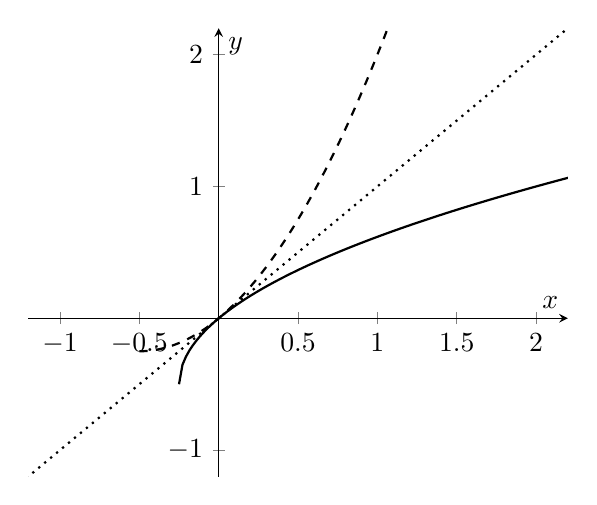
\begin{tikzpicture}
\begin{axis}[axis lines=middle, xlabel=$x$,ylabel=$y$,xmin=-1.2,xmax=2.2,ymin=-1.2,ymax=2.2, samples=150]

\addplot[thick, dashed, color=black,domain=-0.5:3] {x^2+x};
\addplot[thick, color=black,domain=-0.25:3] {(-1+sqrt(1+4*x))/2};
\addplot[thick, dotted, color=black,domain=-2:3] {x};
\end{axis}
\end{tikzpicture}
\end{center}
\caption{\label{gr5} Graf funkcije iz zadatka \ref{invgraph}}
\end{figure}
\end{proof}
\section{Rastav na parcijalne razlomke}

\begin{definition}
\textbf{Racionalna funkcija} je funkcija oblika
$$x\mapsto \dfrac{f(x)}{g(x)},$$
gdje su $f$ i $g$ polinomi i $g\neq 0$ za bar jedan $x\in \mathbb{R}$. Ako je $\st{f}<\st{g}$, onda kažemo da je ona \textbf{prava} racionalna funkcija, a ako je $\st{f}\geq \st{g}$, kažemo da je ona \textbf{neprava}.
\end{definition}

\begin{remark}[O rastavu prave racionalne funkcije na parcijalne razlomke]
\label{partfrac}
Neka su $f$ i $g\neq 0$ polinomi. Svaka prava racionalna funkcija $x\mapsto R(x)=\dfrac{f(x)}{g(x)}$ može se na jedinstven način prikazati kao zbroj parcijalnih razlomaka. Preciznije, zapišimo $g(x)$ u obliku
$$g(x)=(x-x_1)^{k_1}\dots (x-x_s)^{k_s}(x^2+a_1x+b_1)^{l_1}\dots (x^2+a_rx+b_r)^{l_r}.$$
Tada postoje jedinstveni realni brojevi $A_1, \dots, A_{k_1}, D_1,$ $\dots, D_{k_s}, M_1, N_1,$ $ \dots, M_{l_1},$ $ N_{l_1},$ $ \dots R_1,$ $ S_1,$ $\dots, R_{l_r}, S_{l_r}\in \mathbb{R}$ takvi da za sve $x$ iz domene funkcije $x\mapsto R(x)$ vrijedi
\begin{align*}
R(x)&=\dfrac{A_1}{x-x_1}+\dots+\dfrac{A_{k_1}}{(x-x_1)^{k_1}}+\dots+\dfrac{D_1}{x-x_s}+\dots+\dfrac{D_{k_s}}{(x-x_s)^{k_s}} \\
&+\dfrac{M_1x+N_1}{x^2+a_1x+b_1}+\dots+\dfrac{M_{l_1}x+N_{l_1}}{(x^2+a_1x+b_1)^{l_1}}+\dots \\
&+\dfrac{R_1x+S_1}{x^2+a_rx+b_r}+\dots+\dfrac{R_{l_r}x+S_{l_r}}{(x^2+a_rx+b_r)^{l_r}}.
\end{align*}
\end{remark}
Pri rješavanju zadataka trebat će nam još i sljedeći rezultat.
\begin{remark}
\label{poleq}
Neka je $S$ podskup od $\mathbb{R}$ koji se sastoji od svih realnih brojeva, osim možda njih konačno mnogo. Zadane su funkcije $f, g : S\to \mathbb{R}$,
$$f(x)=\sum_{k=0}^n{a_kx^k},\;\;\;g(x)=\sum_{k=0}^m{b_lx^l},$$
gdje su $a_n, b_m\neq 0$. Tada vrijedi $f=g$ ako i samo ako je $m=n$ i $a_j=b_j$ za sve $j=0, 1, \dots, n$.
\end{remark}
Prethodna tvrdnja je zapravo generalizacija teorema o jednakosti polinoma i na one polinome koji nisu definirani na cijelom $\mathbb{R}$.\footnote{U strogom smislu, takve funkcije nisu polinomi, jer ste na predavanju sve polinome definirali na cijelom $\mathbb{R}$, v. \cite{3}.} Međutim, dokaz je potpuno analogan.\footnote{v. \cite{12}, str. 58, 59. Za vježbu pokušajte uočiti što bi trebalo promijeniti u dokazu teorema 1 i 2.}
\begin{exercise}
Rastavite funkciju $x\mapsto \dfrac{1}{(x+2)(x+3)^2}$ na parcijalne razlomke.
\end{exercise}
\begin{proof*}
Prema napomeni \ref{partfrac} znamo da postoje i jedinstveni su brojevi $A$, $B$ i $C$ takvi da za sve $x\in \mathbb{R}\setminus\{-2, -3\}$ vrijedi
$$\dfrac{1}{(x+2)(x+3)^2}=\dfrac{A}{x+2}+\dfrac{B}{x+3}+\dfrac{C}{(x+3)^2}.$$
Želimo odrediti $A$, $B$ i $C$. Pomnožimo li obje strane s $(x+2)(x+3)^2$, proširivanjem dobivamo da za sve $x\in \mathbb{R}\setminus\{-2, -3\}$ vrijedi
$$1=Ax^2+6Ax+9A+Bx^2+5Bx+6B+Cx+2C,$$
odnosno
$$1=(A+B)x^2+(6A+5B+C)x+(9A+6B+2C).$$
Iz prethodnog imamo da su $$P_1, P_2 : \mathbb{R}\setminus\{-2, -3\}\to \mathbb{R},\;P_1(x)=1,\; P_2(x)= (A+B)x^2+(6A+5B+C)x+(9A+6B+2C)$$ jednaki, pa iz napomene \ref{poleq} slijedi
$$\begin{cases}
A+B=0, \\
6A+5B+C=0, \\
9A+6B+2C=1.
   \end{cases}$$
Rješavanjem prethodnog sustava dobivamo $A=1$, $B=-1$ i $C=-1$, pa zaključujemo da je
\[
\pushQED{\qed}
\dfrac{1}{(x+2)(x+3)^2}=\dfrac{1}{x+2}-\dfrac{1}{x+3}-\dfrac{1}{(x+3)^2}.\qedhere
\popQED
\]
\end{proof*}
\begin{exercise}
Dokažite da je funkcija zadana formulom $x\mapsto R(x)=\dfrac{x^3+6x^2+9x+1}{x^2+5x+6}$ injekcija na $\langle -2, \infty\rangle$.
\end{exercise}
\begin{proof}[Rješenje]
Ideja je $R(x)$ prikazati kao sumu jednostavnijih razlomaka, u nadi da ćemo funkciju iz zadatka moći prikazati kao zbroj strogo rastućih funkcija. Dijeljenjem polinoma imamo
$$\dfrac{x^3+6x^2+9x+1}{x^2+5x+6}=x+1+\dfrac{-2x-5}{x^2+5x+6}.$$
Rastavimo $x\mapsto \dfrac{-2x-5}{x^2+5x+6}$ na parcijalne razlomke. Faktorizacijom nazivnika dobivamo $x^2+5x+6=(x+3)(x+2)$. Slijedi da postoje jedinstveni $A$, $B\in \mathbb{R}$ takvi da za sve $x\in \mathbb{R}\setminus\{-2, -3\}$ vrijedi
$$\dfrac{-2x-5}{(x+2)(x+3)}=\dfrac{A}{x+2}+\dfrac{B}{x+3},$$
te množenjem s $(x+2)(x+3)$ dobivamo 
\begin{gather}
\label{partfrac2}
-2x-5=A(x+3)+B(x+2),\;\;\; \forall x\in \mathbb{R}\setminus\{2, 3\}.
\end{gather}
Analogno kao u prethodnom zadatku dobivamo $A, B=-1$. To znači da vrijedi
$$\dfrac{x^3+6x^2+9x+1}{x^2+5x+6}=x+1-\dfrac{1}{x+2}-\dfrac{1}{x+3}$$
za sve $x\in \mathbb{R}\setminus\{-2, -3\}$, pa specijalno i za sve $x\in\langle -2,\infty \rangle$. Kako su $x\mapsto x+1$, $x\mapsto -\dfrac{1}{x+2}$, $x\mapsto -\dfrac{1}{x+3}$ strogo rastuće na $\langle -2,\infty \rangle$, slijedi i da je početna funkcija strogo rastuća na tom intervalu.
\end{proof}
\begin{remark}
Na ovome mjestu bi bilo dobro spomenuti jedan trik koji bi u situacijama poput ove mogao uštedjeti vrijeme. Naime, da bi odredili $A$ i $B$ dovoljno je u (\ref{partfrac2}) uvrstiti $x=-2$ i $x=-3$, respektivno. Međutim, nije odmah očigledno da to možemo, jer u (\ref{partfrac2}) nemamo jednakost polinoma i u točkama $x=2$, $x=3$. 

Tvrdimo da su polinomi jednaki i u tim točkama. Zaista, znamo da svaki polinom koji nije konstanta ima najviše $n$ nultočaka, gdje je $n\in \mathbb{N}$ stupanj polinoma. Kontrapozicijom dobivamo da ako proizvoljan polinom ima beskonačno mnogo nultočaka, onda je on nužno konstanta. No lako vidimo da je jedini polinom koji uopće ima nultočku nul-polinom. 

Posljedica prethodne tvrdnje je sljedeća -- ako su dva polinoma jednaka u beskonačno mnogo točaka, onda su oni jednaki za sve realne brojeve. Zaista, neka su $f$ i $g$ polinomi koji su jednaki u beskonačno mnogo točaka. No tada $f-g$ ima beskonačno mnogo nultočaka, a to znači da je $f-g=0$, odnosno $f=g$. Time smo dokazali tvrdnju. 

Kako su u našem slučaju polinomi $x\mapsto -2x-5$ i $x\mapsto A(x+3)+B(x+2)$ očito jednaki u beskonačno mnogo točaka, oni su sigurno jednaki i u $x=-2$ i $x=-3$, što smo i tvrdili.
\end{remark}
\section{Prirodna domena}
\begin{remark}
Neka je $x\mapsto f(x)$ funkcija zadana formulom. Skup svih $x\in \mathbb{R}$ za koju je $f(x)$ dobro definiran zove se \textbf{prirodna domena} funkcije $f$.
\end{remark}

\begin{exercise}
Odredite prirodnu domenu funkcije $x\mapsto f(x)$, ako je
\begin{itemize}
\item[a)] $f(x)=\sqrt{\log_2(x^2-1)}$,
\item[b)] $f(x)=\arcosh(x^2-4x)+\cth(x-6)$,
\item[c)] $f(x)=\artanh{\sqrt{x}}+\log_2(x+2)$.
\end{itemize}
\end{exercise}
\begin{proof}[Rješenje]
a) Uočimo da je domena od $x\mapsto \log_2{x}$ jednaka $\mathbb{R}^+$, a domena od $x\mapsto \sqrt{x}$ jednaka $[0, \infty\rangle$. Zato trebaju biti zadovoljeni sljedeći uvjeti:
\begin{itemize}
\item $x^2-1>0$,
\item $\log_2(x^2-1)\geq 0$.
\end{itemize}
Prvi uvjet vrijedi ako i samo ako je $x\in \langle-\infty, -1\rangle\cup \langle 1, \infty\rangle$.

Promotrimo drugi uvjet. Uočimo da vrijedi $$\log_2(x^2-1)\geq 0\Leftrightarrow x^2-1\geq 1,$$
za sve $x\in \langle-\infty, -1\rangle\cup \langle 1, \infty\rangle$ (Uvjerite se u to!). No ovo je ekvivalentno tvrdnji $x\in \langle-\infty, -\sqrt{2}\rangle\cup \langle \sqrt{2}, \infty\rangle$. Dakle, domena funkcije $f$ je upravo $$\langle-\infty, -\sqrt{2}\rangle\cup \langle \sqrt{2}, \infty\rangle.$$

b) Uočimo da je domena od $x\mapsto \arcosh{x}$ jednaka $[1, \infty\rangle$, a domena od $x\mapsto \cth{x}$ je jednaka $\mathbb{R}\setminus\{0\}$. Imamo sljedeće uvjete:
\begin{itemize}
\item $x^2-4x\geq 1$,
\item $x-6\neq 0,\text{ odnosno } x\neq 6$.
\end{itemize}
Rješenje nejednadžbe $x^2-4x\geq 1$ je $x\in \langle -\infty, 2-\sqrt{5}]\cup [2+\sqrt{5}, \infty\rangle$, pa je domena
$$\langle -\infty, 2-\sqrt{5}]\cup [2+\sqrt{5}, \infty\rangle\setminus\{6\}.$$

c) Uočimo da je domena od $x\mapsto \artanh{x}$ jednaka $\langle -1, 1\rangle$. Odavde slijedi da trebaju biti zadovoljeni sljedeći uvjeti:
\begin{itemize}
\item $x\geq 0$,
\item $x+2>0,\text{ odnosno }x>-2$,
\item $\sqrt{x}\in \langle -1, 1\rangle$.
\end{itemize}
Primijetimo da drugi uvjet možemo zanemariti. Nadalje, treba vrijediti $\sqrt{x}>-1$ i $\sqrt{x}<1$. $\sqrt{x}>-1$ je istinita za sve realne $x$, pa je možemo zanemariti. Nadalje, vrijedi $\sqrt{x}<1$ ako i samo ako vrijedi $ x<1$. Dakle, domena početne funkcije je $[0, 1\rangle$.
\end{proof}
\begin{exercise}
Odredite sve $x\in \mathbb{R}$ za koje vrijedi
$$\arcsin{\dfrac{\log_2(x+2)}{2}}=\sqrt{-x-\dfrac{7}{4}}-\dfrac{\pi}{2}.$$
\end{exercise}
\begin{proof}[Rješenje]
Prvo bi bilo dobro vidjeti kad su oba izraza definirana. Drugim riječima, trebamo odrediti prirodne domene funkcija $x\mapsto \arcsin{\dfrac{\log_2(x+2)}{2}}$ i $x\mapsto \sqrt{-x-\dfrac{7}{4}}-\dfrac{\pi}{2}$. Lako se vidi da je domena funkcije $x\mapsto \sqrt{-x-\dfrac{7}{4}}-\dfrac{\pi}{2}$ jednaka $\left\langle -\infty, -\dfrac{7}{4}\right]$.

Odredimo domenu funkcije $x\mapsto \arcsin{\dfrac{\log_2(x+2)}{2}}$. Sjetimo se da je domena funkcije $x\mapsto \arcsin{x}$ jednaka $[-1, 1]$. Zato trebaju biti zadovoljeni sljedeći uvjeti:
\begin{itemize}
\item $x+2>0$, odnosno $x>-2$,
\item $\dfrac{\log_2(x+2)}{2}\in [-1, 1]$.
\end{itemize}
Očito za sve $x>-2$ vrijedi $\dfrac{\log_2(x+2)}{2}\in [-1, 1]$ ako i samo ako je
$$-2\leq \log_2(x+2)\leq 2,$$
što je ekvivalentno tvrdnji
$$\dfrac{1}{4}\leq x+2\leq 4,$$
što vrijedi ako i samo ako je $x\in \left[-\dfrac{7}{4}, 2\right]$. Dakle jedini realan broj za kojeg su oba izraza definirana je upravo $\dfrac{7}{4}$. No lako se provjeri da $x\mapsto \arcsin{\dfrac{\log_2(x+2)}{2}}$ i $x\mapsto \sqrt{-x-\dfrac{7}{4}}-\dfrac{\pi}{2}$ poprimaju vrijednost $-\dfrac{\pi}{2}$ za $x=\dfrac{7}{4}$. Zato je to jedino rješenje početne jednadžbe.
\end{proof}
\begin{exercise}
Neka je $x\mapsto f(x)$ funkcija zadana formulom $f(x)=\arccos\left(\tg\left(1+\dfrac{1}{x}\right)\right)$. Odredite prirodnu domenu ove funkcije.
\end{exercise}
\begin{proof}[Rješenje]
Trebaju biti zadovoljeni sljedeći uvjeti:
\begin{itemize}
\item $x\neq 0$,
\item $1+\dfrac{1}{x}\notin \left\{\dfrac{\pi}{2}+k\pi : k\in \mathbb{Z}\right\}$,
\item $\tg\left(1+\dfrac{1}{x}\right)\in [-1, 1]$.
\end{itemize}
Vrijedi $\tg\left(1+\dfrac{1}{x}\right)\in [-1, 1]$ ako i samo ako je
\begin{gather}
\label{4}
1+\dfrac{1}{x}\in \bigcup_{k\in \mathbb{Z}}{\left[-\dfrac{\pi}{4}+k\pi, \dfrac{\pi}{4}+k\pi\right]},
\end{gather}
odnosno ako i samo ako (v. napomenu \ref{unprfam}) postoji $k\in \mathbb{Z}$ takav da je
$$-\dfrac{\pi}{4}+k\pi\leq 1+\dfrac{1}{x} \leq \dfrac{\pi}{4}+k\pi.$$
Primijetimo da (\ref{4}) obuhvaća i činjenicu $1+\dfrac{1}{x}\notin \left\{\dfrac{\pi}{2}+k\pi : k\in \mathbb{Z}\right\}$. Uočimo da je (\ref{4}) ekvivalentno uvjetu
\begin{gather}
\label{5}
-\dfrac{\pi}{4}-1+k\pi\leq \dfrac{1}{x} \leq \dfrac{\pi}{4}-1+k\pi.
\end{gather}
Htjeli bismo odavde dobiti u kojem segmentu se nalazi $x$. Uočimo prvo da su svi intervali $\left[-\dfrac{\pi}{4}-1+k\pi, \dfrac{\pi}{4}-1+k\pi\right]$ podskupovi jednog (i samo jednog) od skupova $\langle -\infty, 0\rangle$ i $\langle 0, \infty\rangle$. Zaista, za $k\geq 1$ vrijedi
$$-\dfrac{\pi}{4}-1+k\pi\geq -\dfrac{\pi}{4}-1+\pi>0$$
i analogno $\dfrac{\pi}{4}-1+k\pi<0$ za $k\leq 0$. Dakle, za $k\geq 1$ imamo $\dfrac{1}{x}>0$, odnosno $x>0$, pa možemo "množiti" s $x$ i $\dfrac{\pi}{4}-1+k\pi$. U tom slučaju dobivamo
$$x\in \bigcup_{k\in \mathbb{Z}}{\left[\dfrac{1}{\dfrac{\pi}{4}-1+k\pi}, \dfrac{1}{-\dfrac{\pi}{4}-1+k\pi}\right]},$$
Analogno, ako je $k\leq 0$, onda također možemo "množiti" s  $x$ i $\dfrac{\pi}{4}-1+k\pi$, ali se pritom mijenja predznak. Analogno dobivamo
$$x\in \bigcup_{k\in \mathbb{Z}\setminus{\mathbb{N}}}{\left[\dfrac{1}{\dfrac{\pi}{4}-1+k\pi}, \dfrac{1}{-\dfrac{\pi}{4}-1+k\pi}\right]},$$
te kako oba uvjeta obuhvaćaju i uvjet $x\neq 0$ (jer su ili oba "ruba" segmenta negativna ili oba pozitivna), slijedi da je prirodna domena početne funkcije upravo 
\begin{align*}
&\bigcup_{k\in \mathbb{N}}{\left[\dfrac{1}{\dfrac{\pi}{4}-1+k\pi}, \dfrac{1}{-\dfrac{\pi}{4}-1+k\pi}\right]}\cup \bigcup_{k\in \mathbb{Z}\setminus{\mathbb{N}}}{\left[\dfrac{1}{\dfrac{\pi}{4}-1+k\pi}, \dfrac{1}{-\dfrac{\pi}{4}-1+k\pi}\right]}\\
&=\bigcup_{k\in \mathbb{Z}}{\left[\dfrac{1}{\dfrac{\pi}{4}-1+k\pi}, \dfrac{1}{-\dfrac{\pi}{4}-1+k\pi}\right]}.\qedhere
\end{align*}
\end{proof}
\begin{remark}
Uočite da smo u prethodnom zadatku primijenili vrlo intuitivnu činjenicu da je za sve familije $\mathcal{F}=\{A_n : n\in \mathbb{Z}\}$, $\mathcal{F}'=\{A_n : n\in \mathbb{N}\}$ i $\mathcal{F}''=\{A_n : n\in \mathbb{Z}\setminus\mathbb{N}\}$,
$$\bigcup_{k\in \mathbb{Z}}{A_n}=\bigcup_{k\in \mathbb{N}}{A_n}\cup \bigcup_{k\in \mathbb{Z}\setminus\mathbb{N}}{A_n}.$$
Dokažimo to! Zaista, vrijedi $\displaystyle x\in \bigcup_{k\in \mathbb{N}}{A_n}\cup \bigcup_{k\in \mathbb{Z}\setminus\mathbb{N}}{A_n}$ ako i samo ako ili postoji $i\in \mathbb{N}$ takav da je $x\in A_i$, ili postoji $j\in \mathbb{Z}\setminus\mathbb{N}$ takav da je $x\in A_j$. Očito, to vrijedi ako i samo ako postoji $k\in \mathbb{Z}$ takav da je $x\in A_k$, tj. $\displaystyle x\in \bigcup_{k\in \mathbb{Z}}{A_n}$.
\end{remark}

\section{Periodične funkcije}

\begin{definition}
Neka je zadana funkcija $f : A\to B$, $A$, $B\subseteq \mathbb{R}$ i $\tau>0$. Kažemo da je $f$ \textbf{periodična s periodom $\tau$} ako za sve $x\in A$ vrijedi $x+\tau \in A$ i $f(x+\tau)=f(x)$. Najmanji od svih perioda, ako postoji, zvat ćemo \textbf{temeljnim periodom}.
\end{definition}

Lako vidimo iz grafova od $\sin$ i $\cos$ da su oni periodični s temeljnim periodom $2\pi$. Nadalje, funkcija $x\mapsto c$, $c\in \mathbb{R}$ je periodična i ona nema temeljni period.
\begin{exercise}
Dokažite da je $x\mapsto \sin{x}$ periodična s temeljnim periodom $2\pi$.
\end{exercise}
\begin{proof}[Rješenje]
Znamo da $x\mapsto \sin{x}$ ima domenu $\mathbb{R}$, pa je tvrdnja o domeni trivijalno zadovoljena za bilo koji $\tau\in \mathbb{R}$. Znamo i da je $$\sin(x+2\pi)=\sin{x},\;\;\; \forall x\in \mathbb{R}.$$ Još preostaje pokazati da je $2\pi$ temeljni period. 

Pretpostavimo da postoji neki period $\tau_0$ takav da je $\tau_0<2\pi$. Tada je $\sin(x+\tau_0)=\sin{x}$. Specijalno, iz definicije za $x=0$ imamo $\sin{\tau_0}=0$. To je moguće ako i samo ako je $$x\in \{k\pi : k\in \mathbb{Z}\}.$$ No kako imamo $0<\tau_0<2\pi$ slijedi nužno $\tau_0=\pi$. No $\pi$ očito nije period, jer je npr. $\sin{\dfrac{\pi}{2}}=1$ i $\sin\left(\dfrac{\pi}{2}+\pi\right)=-1$.
\end{proof}
\begin{exercise}
Funkcija $D : \mathbb{R}\to \mathbb{R}$,
$$D(x)=\begin{cases}
0, & x\in \mathbb{I},\\
1, & x\in \mathbb{Q}
\end{cases}$$
zove se \textit{Dirichletova funkcija}. Dokažite da je ona periodična, ali nema temeljni period.
\end{exercise}
\begin{proof}[Rješenje]
Tvrdimo da je svaki pozitivan $\tau\in \mathbb{Q^+}$ jedan period funkcije $D$. Odavde će biti očito da je $D$ periodična i da nema temeljni period.

Zaista, neka je $x\in \mathbb{R}$ proizvoljan. Tvrdimo da je $x\in \mathbb{Q}$ ako i samo ako je $x+\tau\in \mathbb{Q}$. Zaista, ako je $x\in \mathbb{Q}$, onda je očito $x+\tau\in \mathbb{Q}$. Nadalje, ako je $x+\tau\in \mathbb{Q}$, iz činjenice da je $-\tau\in \mathbb{Q}$ slijedi da je i $(x+\tau)-\tau=x\in \mathbb{Q}$.

Kontrapozicijom slijedi: Ako je $x\in \mathbb{Q}$, onda je $x+\tau\in \mathbb{Q}$, te ako je $x\in \mathbb{I}$ iracionalan, onda je i $x+\tau\in \mathbb{I}$. U oba slučaja imamo $f(x+\tau)=f(x)$ i tvrdnja je dokazana.
\end{proof}
\begin{exercise}
Je li funkcija $x\mapsto x\sin{x}$ periodična?
\end{exercise}
\begin{proof}[Rješenje]
Iz grafa funkcije možemo naslutiti da ona nije periodična.
\begin{figure}[ht]
\begin{center}
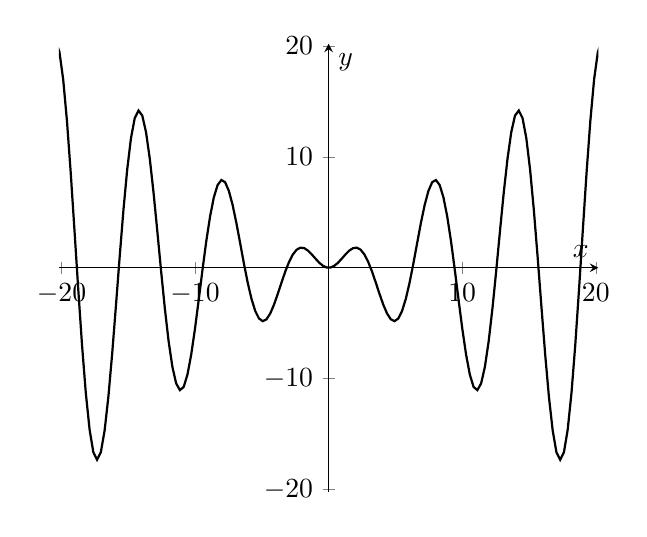
\begin{tikzpicture}
\begin{axis}[axis lines=middle, xlabel=$x$,ylabel=$y$,xmin=-20.2,xmax=20.2,ymin=-20.2,ymax=20.2, samples=150]

\addplot[thick, color=black,domain=-21:21] {x*sin(deg(x))};
\end{axis}
\end{tikzpicture}
\end{center}
\caption{\label{gr6} Graf funkcije $x\mapsto x\sin{x}$}
\end{figure}

Dokažimo tvrdnju. Zaista, pretpostavimo da postoji neki period $\tau>0$. Funkcija je definirana za sve realne brojeve, pa je $x+\tau\in \mathcal{D}(f)$. Po pretpostavci imamo $$(x+\tau)\sin(x+\tau)=x\sin{x},\; \forall x\in \mathbb{R}.$$ 
Specijalno, za $x=-\tau$ imamo $\tau\sin{\tau}=0$, odnosno $\sin{\tau}=0$. To je ekvivalentno sa $\tau\in \{k\pi : k\in \mathbb{N}\}$, gdje je $k\in \mathbb{N}$ jer je $\tau>0$, po definiciji perioda. No to znači da postoji $k\in \mathbb{N}$ takav da je $$(x+k\pi)\sin(x+k\pi)=x\sin{x},\;\forall x\in \mathbb{R}.$$ Ako je $k$ paran, onda je $\sin(x+k\pi)=\sin{x}$. Uzmimo $x$ takav da je $\sin{x}\neq 0$. Tada dijeljenjem sa $\sin{x}$ dobivamo $\pi=0$, kontradikcija! 

Ako je $k$ neparan, onda je $\sin(x+k\pi)=-\sin{x}$. Uzmimo $x$ takav da je $x\in \mathbb{N}$. Zaista, kako je $\pi\in \mathbb{I}$, vrijedi $\sin{x}\neq 0$, jer bi u suprotnom imali $\dfrac{x}{k}=\pi$. Dijeljenjem sa $\sin{x}$ dobivamo $-x-k\pi=x$, odnosno $-\dfrac{2x}{k}=\pi$. Kontradikcija s činjenicom da je $\pi\in \mathbb{I}$! Dakle slijedi $\tau\notin \{k\pi : k\in \mathbb{N}\}$, čime imamo kontradikciju s činjenicom $\tau\in \{k\pi : k\in \mathbb{N}\}$, i time smo dokazali tvrdnju.
\end{proof}
\newpage
\section*{Zadatci za vježbu}
\addtocontents{toc}{\protect\pagebreak[4]}
\subsection*{Pojam funkcije. Crtanje grafa funkcije}
\begin{exercise}
Nacrtajte grafove sljedećih funkcija. (Kada je interval cijeli $\mathbb{R}$, prikažite "najreprezentativniji" dio grafa). 
\begin{itemize}
\item[a)] $f : [-1, 1]\to \mathbb{R}$, $f(x)=x^2+4x+5$,
\item[b)] $f : \mathbb{R}\to \mathbb{R}$, $f(x)=|x+2|-|x|$,
\item[c)] $f : \mathbb{R}\to \mathbb{R}$, $f(x)=(x-2025)^3-2025$.
\item[d)] $f : \mathbb{R}\setminus\{0\}\to \mathbb{R}$, $f(x)=x+\dfrac{1}{x}$.
\end{itemize}
\end{exercise}
\begin{exercise} Promotrite sljedeću sliku.
\begin{figure}[ht]
\begin{center}
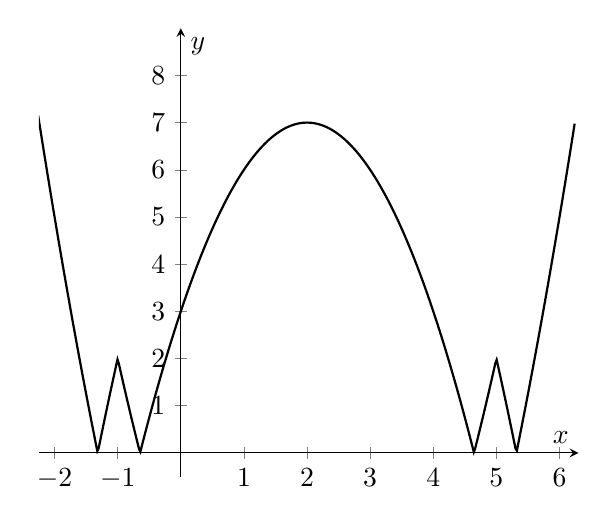
\begin{tikzpicture}
\begin{axis}[axis lines=middle, xlabel=$x$,ylabel=$y$, xtick={-2,-1, 1,2,3,4,5,6}, ytick={1,2,3,4,5,6,7,8},xmin=-2.25,xmax=6.3,ymin=-0.5,ymax=9, samples=400]

\addplot[thick, color=black,domain=-2.26:6.24] {abs(abs(x*x-4*x-5)-2)};
\end{axis}
\end{tikzpicture}
\end{center}
\end{figure}

Ako je poznato da postoje $a, b, c\in \mathbb{R}$, $a\neq 0$ takvi da je graf na slici upravo graf funkcije $f(x)=\left|\left|ax^2+bx+c\right|-2\right|$, odredite neke takve $a, b, c$.
\end{exercise}
\subsection*{Injekcija, surjekcija i bijekcija. Slika i praslika skupa}
\begin{exercise}
Za svaku od sljedećih funkcija odredite je li bijekcija. Ako smatrate da je, dokažite da je, u suprotnom dokažite zašto nije.
\begin{itemize}
\item[a)] $f : \mathbb{R}\to \mathbb{R}$, $f(x)=x^4-x^2$,
\item[b)] $f : \mathbb{R}\to \mathbb{R}$, $f(x)=2x^3+3$.
\item[c)] $f : \mathbb{R}\to [-2, \infty]$, $f(x)=e^x-2$,
\end{itemize}
\end{exercise}
\newpage
\begin{exercise} \textbf{}
\begin{itemize}
\item[a)] Navedite primjer rastuće funkcije $f : \mathbb{R}\to [-1, 1]$.
\item[b)] Navedite primjer padajuće funkcije s $\mathbb{R}$ u $\mathbb{R}$ koja nije ni injekcija ni surjekcija.
\item[b)] Navedite primjer bijekcije $f : \mathbb{R}\to \langle 10, \infty\rangle$.
\item[c)] Navedite primjer bijekcije $f : \langle 10, 20\rangle\to \mathbb{R}$.
\item[d)] Navedite primjer surjekcije $f : \mathbb{R}\to [-1, 0\rangle\cup \langle 0, 1]\cup \{2025\}$.
\item[e)] Navedite primjer surjekcije $f : \mathbb{R}\to \langle -1, 1\rangle \cup \mathbb{N}$.
\end{itemize}
\end{exercise}
\begin{exercise} \textbf{}
\begin{itemize}
\item[a)] Navedite primjer funkcije $f : \mathbb{R}\to \mathbb{R}$ za koju vrijedi $f([0, 5])=[2, 3]$.
\item[b)] Navedite primjer funkcije $f : \mathbb{R}\to \mathbb{R}$ za koju vrijedi $f([0, 5])=[2, 3]$ \textbf{i} $f^{-1}\left(\langle 5, 15]\right)=[-2, -1\rangle \cup \langle 5, 7.5]$.
\item[c)] Postoji li funkcija $f : \mathbb{R}\to \mathbb{R}$ za koju vrijedi $f\left([0, 1]\right)=[1, 2]$ i $f^{-1}\left([1, 3]\right)=[4, 5]$? Dokažite svoje tvrdnje.
\item[d)] Neka je zadana $f : S\to \mathbb{R}$ i neka su $A$, $B\subseteq S$. Dokažite da je $f(A\cap B)=f(A)\cap f(B)$ ako i samo ako je $f$ injekcija.
\end{itemize}
\end{exercise}
\begin{exercise} $(*)$ Neka je $g : \mathbb{R}\to \mathbb{R}$ funkcija takva da je za svaku injekciju $f : \mathbb{R}\to \mathbb{R}$, funkcija $f+g$ također injekcija. Dokažite da je tada $g$ konstanta.
\end{exercise}
\subsection*{Kompozicija funkcija. Inverzna funkcija}
\begin{exercise}
Neka su zadane $f : A\to B$ i $g : B\to C$. Dokažite da ako je $g\circ f$ injekcija, onda je i $f$ injekcija.
\end{exercise}
\begin{exercise}
Neka je $f : \mathbb{R} \to \mathbb{R}$ zadana formulom $f(x)=x^3-2x^2$.
\begin{itemize}
\item[a)] Nacrtajte graf funkcije $f$.
\item[b)] Dokažite da je $f|_{[0, 1]}$ injekcija. Je li $f$ injekcija?
\item[c)] Odredite $f^{-1}\left([0, 9]\right)$ i $f^{-1}\left([2024, 2025]\right)\cap f^{-1}\left([23, 24]\right)$.
\item[d)] Koristeći graf, odredite $f\left([2, 2.2\rangle\right)$.
\end{itemize}
\end{exercise}
\begin{exercise} \textbf{}
\begin{itemize}
\item[a)] Zadana je $f : \mathbb{R}\to \mathbb{R}$, $f(x)=x^4+3|x|^3+4$. Odredite $\mathcal{R}(f)$.
\item[b)] Zadana je $f : [0, \infty\rangle\to \mathbb{R}$, $f(x)=e^{\frac{1-\sqrt{x}}{1+\sqrt{x}}}$. Odredite $f^{-1}\left([1, e]\right)$.
\item[d)] Odredite primjer funkcije $f : \mathbb{R}\to \mathbb{R}$ za koju je $f^{-1}\left([4, 5]\right)=[-3, 2]\cup [6, 7]$.
\end{itemize}
\end{exercise}
\begin{exercise} \textbf{}
\begin{itemize}
\item[a)] Dokažite da je $f : \left[0, \dfrac{\pi}{2}\right]\to [4, 8]$ za koju je $f(x)=\sin^4{x}+3\sin^2{x}+4$ bijekcija i odredite njezin inverz.
\item[a)] Odredite skup $S$ (ako postoji) takav da $f : \mathbb{R}\to S$, $f(x)=\th^3{x}+1$ bude bijekcija.
\item[b)] Neka je $f : \mathbb{R}\to [-2, \infty\rangle$ zadana formulom $f(x)=\abs{\abs{\abs{x}-2}-2}-2$. 
Ispitajte injektivnost, surjektivnost i koristeći graf odredite $f^{-1}\left(\left[\dfrac{1}{2}, 4\right\rangle\right)$.
\end{itemize}
\end{exercise}
\begin{exercise} \textbf{}
\begin{itemize}
\item[a)] Odredite neki $a\in\mathbb{R}$ (ako postoji) takav da je $f : [a, \infty\rangle\to \mathbb{R}$, $f(x)=x^4-2x^2$ injekcija.
\item[b)] Neka su zadane $f, g : S\to \mathbb{R}$. Dokažite ili opovrgnite: Ako su $f$ i $g$ strogo rastuće i ako vrijedi $f(x)\geq 0$ i $g(x)\geq 0$ za sve $x\in S$, onda je i $fg$ strogo rastuća.
\item[c)] Odredite sve $x\in \mathbb{R}$ takve da je $x^3-2x=4$. (Dokažite svoje tvrdnje!)
\end{itemize}
\end{exercise}
\begin{exercise}
Neka je $g : \mathbb{R}\to \mathbb{R}$ funkcija takva da za funkciju $h : \mathbb{R}\to \mathbb{R}$, $h(x)=g^9(x)+2g^3(x)+1$, vrijedi $h\left([0, 2]\right)=[-2, 4]$. Odredite $g\left([0, 2]\right)$.
\end{exercise}
\begin{exercise} $(*)$
Neka je $f : \mathbb{R}\to \mathbb{R}$ dana izrazom $f(x)=\dfrac{x}{\sqrt{1+x^2}}$. Neka je $f_n(x)=\underbrace{f(f(\dots f(x))\dots)}_\text{$n$ puta}$. Izračunajte $f_{2024}(2024)$ i pokažite da je $f_{2024}$ injekcija.
\end{exercise}
\begin{exercise} $(*)$
Zadana je $f : \mathbb{R}\to \mathbb{R}$,
$$f(x)=(x+2)(x+3)(x+7)(x+8)$$
Odredite $\mathcal{R}(f)$.
\end{exercise}
\begin{exercise} $(*)$ Izračunajte
$$\arctg{\dfrac{1}{2}}+\arctg{\dfrac{1}{8}}+\arctg{\dfrac{1}{18}}+\dots+ \arctg{\dfrac{1}{2\cdot 2024^2}}.$$
\end{exercise}
\begin{exercise} $(**)$
Može li se funkcija $x\mapsto x\cos(x^3-x)$ prikazati kao kompozicija konačno mnogo funkcija $x\mapsto -x$, $x\mapsto x\sin{x}$, $x\mapsto \sh{x}$, $x\mapsto x^3+x$? Dokažite.
\end{exercise}
\subsection*{Rastav na parcijalne razlomke}
\begin{exercise}
Rastavite sljedeće funkcije na parcijalne razlomke (po potrebi prvo funkciju prikazati kao zbroj polinoma i prave racionalne funkcije). 
\begin{itemize}
\item[a)] $x\mapsto \dfrac{x^3+2x+3}{x^3-x}$,
\item[b)] $x\mapsto \dfrac{1}{x^3+1}$.
\end{itemize}
\end{exercise}
\begin{exercise}
Zadana je $f : \mathbb{R}\setminus\{-1\}\to\mathbb{R}$,
$$f(x)=\dfrac{x^3+6x^2+12x+9}{(x+1)^3}.$$
Odredite $f\left([0, 2]\right)$.
\end{exercise}
\begin{exercise} $(*)$ \textbf{}
Zadan je sustav jednadžbi
$$\begin{cases}
A + C&=9,\\
 3A + B + C + D&=5,\\
 2A + 4B - 2C + E&=7,\\
 -2A + 6B - 2C - 2D - E + F&=4,\\
 -3A + 4B + C - E - 2F&=6,\\
 -A + B + C + D + E + F&=3
   \end{cases}$$
Dokažite (bez korištenja rezultata iz linearne algebre i bez rješavanja sustava) da ovaj sustav ima jedinstveno rješenje, tj. da postoje jedinstveni $A, B, C, D, E, F\in \mathbb{R}$ za koje vrijedi sustav jednadžbi.
\end{exercise}
\subsection*{Prirodna domena}
\begin{exercise}
Odredite prirodnu domenu sljedećih funkcija.
\begin{AutoMultiColItemize}
\item[a)] $x\mapsto \mathrm{arch}\left(\arccos{\dfrac{x-1}{x+2}}+1\right)$,
\item[b)] $x\mapsto \dfrac{1}{\sqrt{\dfrac{1}{x^2}-\dfrac{3}{x}-4}}$
\item[c)] $x\mapsto \arcsin\left(\sqrt{x+2}-\sqrt{x+1}\right)$,
\item[d)] $x\mapsto \sqrt{1+\log\lfloor x^2-1\rfloor},$
\item[e)] $x\mapsto \ln\left(\dfrac{1}{\sin{x}}-2\cos{x}\right).$
\end{AutoMultiColItemize}
\end{exercise}
\newpage
\begin{exercise} Navedite primjer elementarne funkcije čija je prirodna domena:
\begin{AutoMultiColItemize}
\item[a)] $[1, \infty\rangle \setminus \{2\}$,
\item[b)] $\langle 1, \infty\rangle \setminus{\mathbb{N}}$,
\item[c)] $\langle -\infty, 2]\cup [3, \infty\rangle$,
\item[d)] $\mathbb{N}$,
\item[e)] $\langle 0, \infty\rangle\setminus\{2025^n : n\in \mathbb{N}\}$.
\end{AutoMultiColItemize}
(\textbf{Uputa:} Elementarne funkcije su sve one funkcije koje se mogu dobiti pomoću konačnog broja operacija zbrajanja, množenja, oduzimanja, dijeljenja i kompozicije iz potencija, eksponencijalnih, hiperbolnih, trigonometrijskih funkcija i njihovih inverznih funkcija -- korijena, logaritamskih, area i arkus funkcija).
\end{exercise}
\begin{exercise} \textbf{}
\begin{itemize}
\item[a)] Zadana je elementarna funkcija $f : \mathbb{R}\to \mathbb{R}$. Dokažite da je za svaki konačan skup $S\subseteq \mathbb{R}$ restrikcija $f|_{\mathbb{R}\setminus{S}}$ također elementarna funkcija.
\item[b)] Dokažite da za svaki konačan skup $S\subseteq \mathbb{R}$ postoji elementarna funkcija čija je prirodna domena $S$.
\end{itemize}
\end{exercise}
\subsection*{Periodične funkcije}
\begin{exercise}
Je li $x\mapsto \sin^2{x}$ periodična? Ako je, koji joj je temeljni period? Dokažite sve svoje tvrdnje.
\end{exercise}
\begin{exercise}
Zadana je funkcija $f : \mathbb{R}\to \mathbb{R}$,
$$f(x)=\begin{cases}
-x+5n+1 & \text{za } x\in [5n, 5n+1],\, n\in \mathbb{N},\\
0 & \text{za } x\in [5n+1, 5n+2],\, n\in \mathbb{N},\\
-x+5n+2 & \text{za } x\in [5n+2, 5n+3],\, n\in \mathbb{N},\\
x-5n-4 & \text{za } x\in [5n+3, 5n+5],\, n\in \mathbb{N},
\end{cases}$$
Dokažite da je $f$ periodična i odredite joj temeljni period. Dokažite sve svoje tvrdnje.
\end{exercise}